% Options for packages loaded elsewhere
\PassOptionsToPackage{unicode}{hyperref}
\PassOptionsToPackage{hyphens}{url}
%
\documentclass[
]{book}
\usepackage{lmodern}
\usepackage{setspace}
\usepackage{amssymb,amsmath}
\usepackage{ifxetex,ifluatex}
\ifnum 0\ifxetex 1\fi\ifluatex 1\fi=0 % if pdftex
  \usepackage[T1]{fontenc}
  \usepackage[utf8]{inputenc}
  \usepackage{textcomp} % provide euro and other symbols
\else % if luatex or xetex
  \usepackage{unicode-math}
  \defaultfontfeatures{Scale=MatchLowercase}
  \defaultfontfeatures[\rmfamily]{Ligatures=TeX,Scale=1}
\fi
% Use upquote if available, for straight quotes in verbatim environments
\IfFileExists{upquote.sty}{\usepackage{upquote}}{}
\IfFileExists{microtype.sty}{% use microtype if available
  \usepackage[]{microtype}
  \UseMicrotypeSet[protrusion]{basicmath} % disable protrusion for tt fonts
}{}
\makeatletter
\@ifundefined{KOMAClassName}{% if non-KOMA class
  \IfFileExists{parskip.sty}{%
    \usepackage{parskip}
  }{% else
    \setlength{\parindent}{0pt}
    \setlength{\parskip}{6pt plus 2pt minus 1pt}}
}{% if KOMA class
  \KOMAoptions{parskip=half}}
\makeatother
\usepackage{xcolor}
\IfFileExists{xurl.sty}{\usepackage{xurl}}{} % add URL line breaks if available
\IfFileExists{bookmark.sty}{\usepackage{bookmark}}{\usepackage{hyperref}}
\hypersetup{
  pdftitle={Designing and Building Data Science Solutions},
  pdfauthor={Jonathan Leslie; Neri Van Otten},
  hidelinks,
  pdfcreator={LaTeX via pandoc}}
\urlstyle{same} % disable monospaced font for URLs
\usepackage{longtable,booktabs}
% Correct order of tables after \paragraph or \subparagraph
\usepackage{etoolbox}
\makeatletter
\patchcmd\longtable{\par}{\if@noskipsec\mbox{}\fi\par}{}{}
\makeatother
% Allow footnotes in longtable head/foot
\IfFileExists{footnotehyper.sty}{\usepackage{footnotehyper}}{\usepackage{footnote}}
\makesavenoteenv{longtable}
\usepackage{graphicx,grffile}
\makeatletter
\def\maxwidth{\ifdim\Gin@nat@width>\linewidth\linewidth\else\Gin@nat@width\fi}
\def\maxheight{\ifdim\Gin@nat@height>\textheight\textheight\else\Gin@nat@height\fi}
\makeatother
% Scale images if necessary, so that they will not overflow the page
% margins by default, and it is still possible to overwrite the defaults
% using explicit options in \includegraphics[width, height, ...]{}
\setkeys{Gin}{width=\maxwidth,height=\maxheight,keepaspectratio}
% Set default figure placement to htbp
\makeatletter
\def\fps@figure{htbp}
\makeatother
\setlength{\emergencystretch}{3em} % prevent overfull lines
\providecommand{\tightlist}{%
  \setlength{\itemsep}{0pt}\setlength{\parskip}{0pt}}
\setcounter{secnumdepth}{5}
\usepackage{booktabs}

\usepackage{color}
\usepackage{framed}
\setlength{\fboxsep}{.8em}

\newenvironment{smaller}{}

\newenvironment{infobox}{
  \definecolor{shadecolor}{rgb}{0, 0, 0}  % black
  \color{white}
  \begin{shaded}}
 {\end{shaded}}
\usepackage[]{natbib}
\bibliographystyle{apalike}

\title{Designing and Building Data Science Solutions}
\author{Jonathan Leslie \and Neri Van Otten}
\date{2020-08-01}

\begin{document}
\maketitle

{
\setcounter{tocdepth}{1}
\tableofcontents
}
\setstretch{1.5}
\hypertarget{welcome}{%
\chapter*{Welcome}\label{welcome}}
\addcontentsline{toc}{chapter}{Welcome}

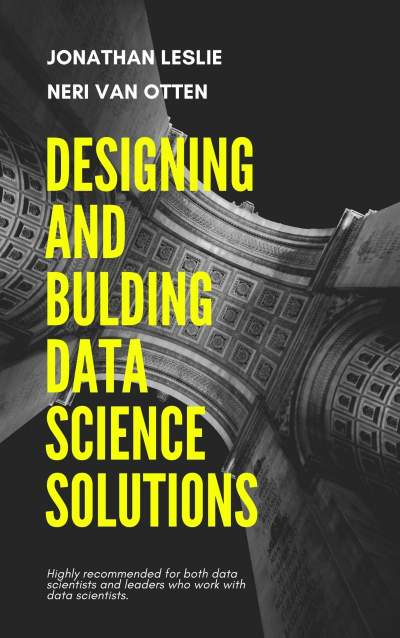
\includegraphics[width=0.5\linewidth,style="float:right; padding:10px"]{figures/Designing and bulding data science solutions seo}

Data science is a dynamic field that, when successful, can have a game-changing impact on a business. Yet designing and delivering a successful data science project can be difficult. Indeed, in a recent \href{https://www.gartner.com/en/newsroom/press-releases/2018-02-13-gartner-says-nearly-half-of-cios-are-planning-to-deploy-artificial-intelligence}{Gartner study}, 85 percent of all data science projects fall short of expectations. The main cause of failure was found to be that replacing legacy systems and associated processes is not easy. Other found issues revolved around not having the right data for the project or not having the right talent. This grim statistic underscores the fact that, for a business, getting started on a data science journey can be risky and daunting.

With this guide, we wish to de-risk the process and help practitioners succeed by providing a step-through guide on how to best tackle the entire process from designing to delivering a successful project. This guide can also be useful for managers, executives and project managers, they will gain insight into how the entire data science project process works.

When building groundbreaking systems or conducting cutting-edge research, one can never be sure where the work will take you. As a data scientist, you can never take all of the uncertainty and risk away. But you CAN approach your projects in a sensible way that can give your projects the best chances of success.

This guide covers our approach. It includes two different frameworks: one for evaluating project success and the other for navigating a data science project lifecycle. We use this system in our work and have found it to be invaluable in helping us to avoid common pitfalls and to give our projects the best chances for impactful outcomes. We hope it is useful to you as well.

\hypertarget{about-us}{%
\section*{About us}\label{about-us}}
\addcontentsline{toc}{section}{About us}

Your authors have each worn many hats: data scientists, project managers, mentors and consultants. We met via the \href{http://www.s2ds.org/}{S2DS} programme, where we worked together as project mentors.

Like many data scientists, we have both come to the field via routes in other disciplines. Jonathan Leslie obtained his PhD in Biology from the University of London, studying blood vessel formation at the Cancer Research UK London Research Institute. After 22 years in biomedical research, he turned to data science and founded a freelance consultancy business. In 2017 he joined \href{https://www.pivigo.com}{Pivigo}, where he is now the Director of Data Science. He is passionate about promoting open-source software and routinely volunteers as a mentor in the R-programming and data science communities.

Neri Van Otten holds a M.Sc. in Computer Science Engineering from Ghent University where she wrote her thesis on optimising energy usage in electrical vehicles by training online personalised deep neural networks. In her 8 years of professional data science experience, she has worked at start-ups, a hedge fund and as an independent data science consultant helping a wide variety of different companies. Technically, she focuses mainly on optimising/scaling machine learning systems to utilise data in real-time, researching deep learning solutions and building NLP (Natural Language Processing) applications. At the moment, she leads the data science efforts at \href{https://www.sourcebreaker.com/}{SourceBreaker}, runs her own deep learning start-up \href{https://www.spotintelligence.com/}{Spot Intelligence} and mentors (aspiring) data scientists. She is passionate about diversity and education and regularly teaches machine learning.

We have designed and executed hundreds of projects using data science, machine learning and artificial intelligence (AI), most of which we would consider ``successful'' (you can read much, much more on the topic of ``success'' in Chapter \ref{levels}). We have also made countless mistakes along the way and have done our best to learn from them. Designing projects, ensuring stakeholder buy-in and delivering successful, relevant outcomes is a difficult task, and it doesn't come naturally to anyone. We hope that you can benefit from the mistakes we have made and the learnings we have acquired in our careers.

\hypertarget{acknowledgements}{%
\section*{Acknowledgements}\label{acknowledgements}}
\addcontentsline{toc}{section}{Acknowledgements}

We would like to thank several people who have contributed to this work. Without you, this would never have happened. We thank Andras Szabo and Kim Nilsson, who spent many hours carefully reading our drafts and providing invaluable feedback. We would also like to thank Ole Moeller Nilsson, Maryam Qurashi, Mandeep Soor, Jason Muller, Neil Forest and Deepak Mahtani for their many suggestions and useful comments. We are especially grateful to our families for their patience and support: Mariam Orme, Daryan Leslie, Zara Leslie (for Jon) and Thea Van Otten, Paul Van Otten and Hilde De Boeck (for Neri).

Copyright © 2020 Jonathan Leslie and Neri Van Otten

\hypertarget{introduction}{%
\chapter{Introduction}\label{introduction}}

The past decade has seen an explosion of technological innovations, perhaps none of which more seismic for both businesses and individuals than the field of data science. Indeed, the ability to apply advanced analytics to business challenges can be exciting, fruitful and fun. With recent advances in computational capabilities and cost-effective data collection and storage solutions, applying data science to business challenges is now within the reach of most business owners.

Getting started with data science can be daunting, and for the non-specialist, exactly how to begin a data science journey can be unclear. Just like software engineering projects, data science projects require specific design strategies. Our personal experience designing data science projects in a wide range of industries and sectors has given us an understanding of how to make this journey successful and how to work with stakeholders to identify the most impactful business questions and formulate scientific approaches to answer them.

In this book, we share our learnings about sensible approaches to designing data science projects. We offer a framework that we have found to be useful in ensuring successful project outcomes and walk the reader through the process of using this framework for their own data science endeavours. Our goal is to provide a resource that data science practitioners can use in their work and give business leaders an insight into the steps that go into building a data science project from scratch.

\hypertarget{the-challenges-when-embarking-on-a-data-science-project}{%
\section{The challenges when embarking on a data science project}\label{the-challenges-when-embarking-on-a-data-science-project}}

For data scientists who are new to the field, perhaps the single most challenging aspect of the role is not technical, but rather conceptual: learning how to design a successful data science project. Often this means breaking down a complex business case into concrete objectives and specific questions. In our roles as mentors and project managers, we too-often see data scientists attack an analysis without first identifying the underlying questions. These can be specific questions about the scientific approach -- ``What is the hypothesis of this experiment?'' or ``What statistical question am I asking my model to answer?'' -- to more general ones such as, ``Why are we doing this?'', ``What is an ideal outcome?'', ``What would constitute a failure?'' or ``What is the business problem we are trying to solve?'' As we tell our mentees, this approach is like building a house without a blueprint: you might hammer together some bits of wood in a useful way, but without understanding the objectives of the project as a whole, success is essentially impossible.

Project design is difficult: it can be loosely structured and often has no single correct answer. This can often be disorienting. How best to approach this task has been considered and discussed often, and many learnings have been derived from the methodologies found in fields such as product design or design engineering. For an excellent discussion of this topic, we recommend episodes 63 - 70 of the podcast \href{http://nssdeviations.com/}{Not So Standard Deviations}, in which hosts Roger Peng and Hilary Parker discuss the Nigel Cross book \href{https://www.amazon.co.uk/Design-Thinking-Understanding-Designers-Blac14/dp/1847886361/ref=sr_1_2?keywords=Nigel+Cross+book+Design+Thinking\&qid=1576333690\&sr=8-2}{Design Thinking} and draw parallels to applications in data science.

We often think of data science as a process by which we frame a business problem as a scientific question and apply scientific methodologies to answer that question and derive insights. But how do we identify the business question in the first place? As a data scientist, a good first step is to ask different stakeholders. Yet in our experience, this can often be an unsatisfying approach: more often than not, the stakeholders (clients or managers) will not have a clearly-defined business problem or a concrete objective for the project. We believe our framework can help drive this conversation, setting the stage for well-planned project design and giving projects the best chances for success.

\hypertarget{a-note-on-data-science-machine-learning-and-artificial-intelligence}{%
\section{A note on data science, machine learning and artificial intelligence}\label{a-note-on-data-science-machine-learning-and-artificial-intelligence}}

``Data science'', ``machine learning'' and ``artificial intelligence'' are terms that can be used in imprecise ways and can have overlapping meanings. Many will be familiar with the phenomenon of a job advertisement that is billed as a data scientist role but in reality, is more of a data analyst or an IT specialist. AI is perhaps the most liberally-used of the terms, sure to increase one's chances of writing a successful grant application or tender for a piece of work. It is safe to say that all of these terms can be susceptible to over-hype, and the choice of which to use often appears as a matter of marketing.

But there are differences between them and it's important to understand what those differences are. One of our \href{http://varianceexplained.org/r/ds-ml-ai/}{favourite discussions} about how these terms relate to one another comes from David Robinson:

\begin{itemize}
\tightlist
\item
  \textbf{Data science} produces \textbf{insights}
\item
  \textbf{Machine learning} produces \textbf{predictions}
\item
  \textbf{Artificial intelligence} produces \textbf{actions}
\end{itemize}

To expand on this slightly, the goal of data science work is to gain insights and understanding into data. While the numerical patterns revealed may be clear and objective, the way these findings are interpreted requires a human in the loop. One way it differs from machine learning is that data science doesn't necessarily involve modelling. We would also argue that it doesn't necessarily involve coding or programming: there are plenty of data scientists that combine domain expertise with statistical inference using spreadsheets to acquire valuable insight.

Machine learning extends data analytics into the realm of predictive modelling. This can be done in a highly automated way, although no machine learning system should be allowed to impact decision-making without a human in the loop. Machine learning models can range in complexity and interpretability. For example, linear regression is at the straight-forward end of the spectrum, so much so that many do not consider it machine learning at all. Deep learning models reside at the opposite end of the spectrum, with inner workings that are so opaque that it is essentially impossible to understand how the model makes its predictions. The difference between data science and machine learning is not black and white but rather a spectrum of two overlapping domains.



\begin{center}

\begin{figure}
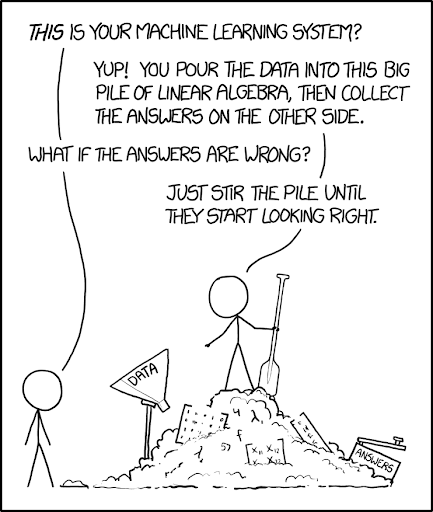
\includegraphics[width=0.5\linewidth]{figures/xkcd} \caption{xkcd.com Machine Learning}\label{fig:xkcd-fig}
\end{figure}

\end{center}

Artificial Intelligence is the most common term that is most widely understood but is possibly also the hardest to distinguish between. Everyone will have their view on this but to distinguish it from the other two terms we will define artificial intelligence as an actional application. This can be anything from robotics used in industries, chatbots providing customer service to game-playing algorithms using reinforcement learning.

For the sake of simplicity, we have chosen to use the term ``data science'' throughout this book as this most accurately represents the type of projects we tackle. In most cases, the reader can substitute the term with ``machine learning'' or ``artificial intelligence'' without losing the message of the text.

\hypertarget{our-framework}{%
\section{Our framework}\label{our-framework}}

Our framework has two related components: \textbf{project execution} and \textbf{project evaluation}. While the temptation may be to view these in series, we have found that these components are intertwined; each has use on its own, but the framework yields the best results when they are used together. In the following chapters, we outline these components, counterintuitively starting with evaluation and then moving on to execution. Why do we start with evaluation? We have found that thinking about what you want the final successful project to look like can help in planning how to get there. In short, we recommend starting with a zoomed-out view of the project as a whole and the context into which it fits before considering the details of how you might get there. We can think of the analogy of taking a road-trip across the country: a sensible approach is to first think about what you want to get out of the journey and what are the major milestones you want to achieve before determining exactly which roads you will take to get there. This has echoes in Test Driven Development (TDD), a common approach to software development in which one first defines the criteria that the final code should adhere to and creates the corresponding tests before writing the actual code.

\hypertarget{organisation-of-this-book}{%
\section{Organisation of this book}\label{organisation-of-this-book}}

This book is divided into two parts. In Part 1 we discuss our approach to designing and executing data science projects. Chapter \ref{levels} covers the four levels of project evaluation in more detail and provides examples of how to assess each. In Chapter \ref{phases} we move on to the phases of project delivery. Two of these phases are then explored in more detail: Project Definition (Chapter \ref{definition}) and Project Execution (Chapter \ref{execution}).

Part 2 focuses on offering more concrete, practical advice. In Chapter \ref{example} we provide an example of a project proposal that we might use when working with a client to define a project. Chapter \ref{consulting} is primarily aimed at independent contractors/freelancers and covers how to build up a client base and find work. Chapter \ref{help} lists some useful resources for where you can find help in the wider data science community.

\hypertarget{part-part-i}{%
\part*{Part I}\label{part-part-i}}
\addcontentsline{toc}{part}{Part I}

\hypertarget{levels}{%
\chapter{What success looks like: the four levels of project evaluation}\label{levels}}

When approaching a data science project, we often look to the end: knowing what a successful outcome would look like is a good way to determine the direction of a project and the steps required to get there. The idea is that if you meet those criteria -- if you deliver something that resembles this desired outcome -- you have succeeded. However, while faithful production of the agreed-upon deliverables is indeed important, this is often only part of a much larger picture.

In early conversations with a stakeholder, you may have agreed upon a certain set of outcomes and deliverables for the project based on the circumstances and understanding at the time. However, circumstances can change. Similarly, simply because you have achieved a predetermined goal for a project does not necessarily mean that this goal is the best outcome for the business. Part of our jobs as data scientists, especially if tasked with designing a project, is to understand what the business needs and help stakeholders see what is the most beneficial. Thus, simply focusing on deliverables falls short when assessing how successful a project has been. Moreover, often in a data science project, we make unexpected discoveries. If we view these solely through the lens of agreed project objectives they could be considered mistakes or shortcomings, however, the unexpected outcomes are often the most valuable to the business.

Eskander Howsawi and colleagues have proposed a framework for evaluating project success that has four levels, termed ``context'', ``business'', ``product'' and ``project process'' (\citet{Howsawi}; Figure \ref{fig:eval-levels}). In our approach to data science project design, we have found striking parallels to the Howsawi framework. (For a more detailed explanation of these levels and this framework, we recommend \href{https://doi.org/10.5130/.v1i0.3865}{reading the paper}.)



\begin{figure}
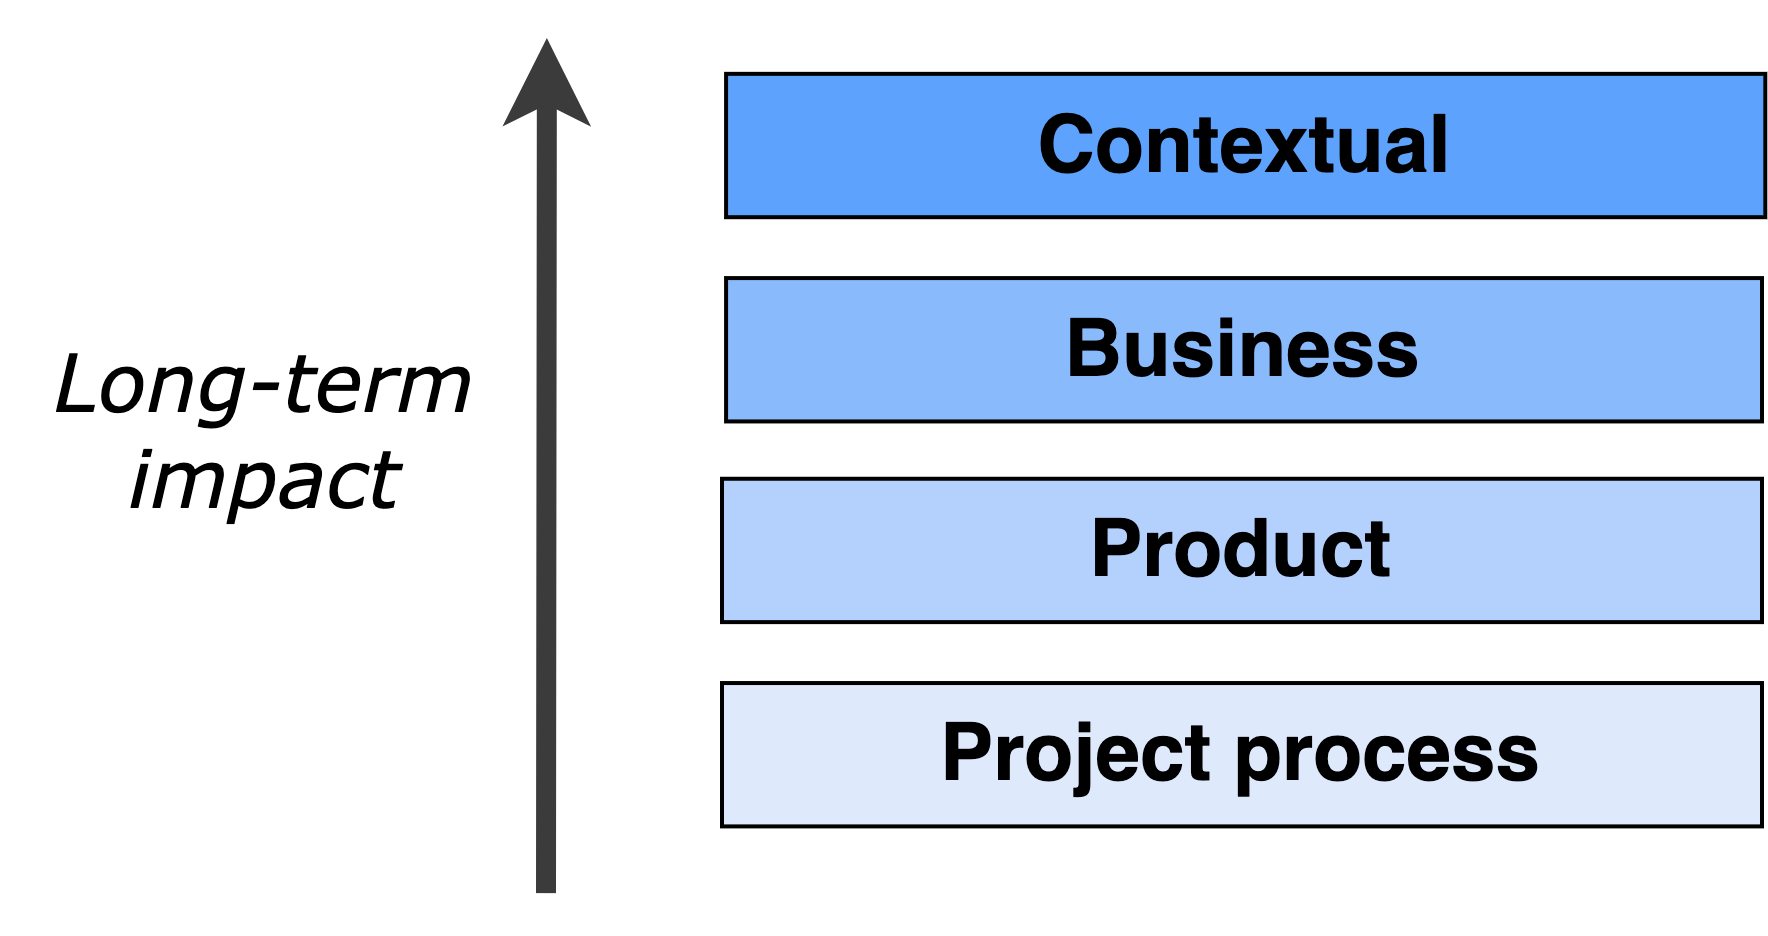
\includegraphics[width=0.7\linewidth]{figures/Figure_1-eval_levels} \caption{\textbf{The four levels of project evaluation}. We evaluate project outcomes at four levels: project process (relating to the execution of the project), product (relating to the delivered final product), business (related to what value the project brings to the business) and contextual (related to circumstances surrounding the project). The higher levels (contextual, business) are more abstract, but also have more relevance to the business value of the work. We recommend you consider all of these when defining, and evaluating, a project. (Adapted from Eskander Howsawi and colleagues.)}\label{fig:eval-levels}
\end{figure}

In the sections below we discuss each of these levels in detail. If you are involved with defining and scoping a project, we strongly recommend you think carefully about how your proposed work satisfies each of these levels. As a consultant, this will be an important part of your role and an important step in developing a project that has real value to its stakeholders. Even if your specific role does not involve project design, we recommend you take the time to consider these levels at both the beginning and the end of a project: if nothing else, it's a good thought exercise that will be important if you are ever involved in project design.

\hypertarget{contextual-level}{%
\section{Contextual level}\label{contextual-level}}

The first and highest level of the project evaluation framework is termed contextual and is the most abstract. This relates to the circumstances surrounding a project and the externalities that affect it. While considering this may seem beyond the remit of the data scientist's role, this level is arguably the most impactful: if a project delivers business value, but the circumstances upon which that value is based change, the realised value may change dramatically. Consider, for example, how Brexit may affect UK businesses -- project outcomes that may have been valuable in 2016 may not hold up after the UK leaves the European Union. Similarly, the COVID-19 pandemic has had seismic effects on many businesses, changing how they operate and the landscape of business opportunities before them. Projects aimed at pre-COVID business cases may no longer have contextual relevance. Understanding and adjusting for these changing circumstances helps ensure that your work is topical, relevant and impactful.

Contextual considerations often are related to business strategy, a good understanding of which is key when designing a project that is going to have an impact well into the future. A company's business strategy describes its vision, culture and image. At its core is an understanding of the business's goals and how its leaders intend to achieve those goals. Naturally, business goals are often centred around performance: attracting customers, increasing profits and reducing costs are almost always major driving forces. But the strategy can also extend beyond that to include things such as organisational culture, brand and image and the company's place in the wider community. It is important to note that the underlying goals driving strategy can vary across sectors. For example, the goals of a government agency will surely be very different from those of private-sector or not-for-profit organisations.

Understanding an organisation's strategy will help you to more clearly see how a data science project fits in. Often such projects are part of an overall move towards innovation, so it can be helpful to clarify what the business is hoping to achieve with that initiative. In our experience, we generally turn to several key questions that can help paint a picture of what the business strategy is:

\begin{itemize}
\tightlist
\item
  What are your business drivers and your strategic imperatives?
\item
  What are the main pain points or challenges in delivering your strategy?
\item
  Who are your competitors and what do you think you need to do to stay or get ahead of them?
\item
  Where do you think you may be missing opportunities?
\item
  Do you have any particular business objectives in mind, such as increasing revenue, reducing costs or improving your products or services?
\item
  Do you have any ongoing data science work already? What is its focus, and how does the current project fit into it?
\end{itemize}

These questions are ones that we, ourselves, often use to help understand the context of the project. They are gleaned from several existing frameworks that can help you to identify the business strategy. We have highlighted a few below.

\hypertarget{swot-analysis}{%
\subsection{SWOT analysis}\label{swot-analysis}}

SWOT (Strengths, Weaknesses, Opportunities and Threats) analysis is a simple, yet powerful tool that is often used to develop a business strategy. While your job as a data scientist or a consultant is not to define your client's overall business strategy, the exercise of going through a SWOT analysis can help you to understand how the company views its position in the market. In short, this analysis allows you to identify internal capabilities (strengths and weaknesses) and external factors (opportunities and threats) to understand the business's competitive advantage and the factors that are favourable or unfavourable to achieving its objectives. LivePlan has an excellent \href{https://www.liveplan.com/blog/what-is-a-swot-analysis-and-how-to-do-it-right-with-examples/}{blog post} that provides an overview of the process along with an example and questions to help drive the conversation.

\hypertarget{porters-five-forces}{%
\subsection{Porter's Five Forces}\label{porters-five-forces}}

Porter's Five Forces framework has echoes in the SWOT analysis described above. Indeed, it's originator, Micheal E. Porter, developed it in reaction to SWOT analysis, which he felt fell short in analyzing competition of a business. It is generally used to assess an industry in terms of its potential for profitability. While this framework can be a powerful tool, in our experience it is less useful in identifying the contextual environment of how data science, or technical innovation in general, fits into a business's strategy. Nevertheless, we mention it here for the benefit of those readers who would like to learn more.

\hypertarget{pestel-analysis}{%
\subsection{PESTEL Analysis}\label{pestel-analysis}}

PESTEL analysis is used to understand the external forces that an organisation faces. The acronym stands for Political, Economic, Social, Technological, Environmental and Legal. The premise is that organisations that are more tuned-in to the changes in these forces will be better positioned to compete. It is often used in conjunction with a SWOT analysis and, when used well, allows an organisation to not only identify these relevant forces but also to assess the potential impact that they may have.

These tools can help give you a better understanding of the circumstances and business motivations driving an organisation's decision to embark on a data science project. You don't necessarily have to go through the formality of a consultation session or a workshop with your client to understand a project's wider context, but our very strong advice is to at least go through the exercise of considering some of the questions we have provided. It will give you a better understanding of how your work fits into the business as a whole and will demonstrate to your client that you are willing to take the time to fully understand the forces that drive their decisions. Usually, your client is looking to you to guide them on their data science journey, and knowing the larger context of your work will go a long way to ensuring that the outcome is relevant and valuable.

\hypertarget{business-level}{%
\section{Business level}\label{business-level}}

The second level of the framework corresponds to the business. In short, this describes how much value the project brings to the business. Unlike concrete, tangible deliverables, business value can be hard to measure. Success on this level may not be realised immediately, but rather may only be understood well after the project has been completed.

How does one plan for business-level success when designing a project? This is a complicated question with no single right answer, however, this is often where the creative beauty of project design comes into play. To do this well, you will want to engage with stakeholders to identify opportunities for business value based on an understanding of the organisation's strategy, therefore the identification of business-level goals should be thought of as a collaborative effort between the data scientist and the business partner.

Naturally, projects must be feasible to generate business value. Thus when defining the business case in Phase 1 (Chapter \ref{phases}), you will often find yourself moving between high-level discussions about what sorts of outcomes would be useful to the organisation and more concrete discussions about feasibility in terms of objectives, budget, data availability and appetite for risk. We discuss ways to drive this conversation during the stages of project design in Chapter \ref{phases}.

In the best cases, the business value generated from a project can be expressed in concrete terms: increased revenue, time saved or measurable increases in customer satisfaction are a few examples. Exactly how a project's outcome results in changes to these values are often confounded by other factors. In other words, your data science project will likely be one of many factors that, collectively, affect revenue or costs. Therefore, defining KPIs (Key Performance Indicators) that can accurately and quantifiably assess the impact of your work in an isolated environment will help when assessing your project's value at the business level. We recommend that you work with your client or internal stakeholders to identify the relevant KPIs during the design stages of your project. This is covered in Chapter \ref{KPIs} in more detail. For another discussion of how to consider business objective in data science projects, we recommend \href{https://www.oreilly.com/radar/what-you-need-to-know-about-product-management-for-ai/}{this piece by Peter Skomoroch and Mike Loukides}.

Sometimes the business value from a project cannot be measured objectively. Indeed, the value of exploratory and proof-of-concept projects is often in the knowledge generated or insights into the potential for future investments. For example, many of our clients undertake proof-of-concept projects to answer specific questions such as, ``Is it worth it for us to invest in hiring a data science team to take this work further?'' While it's hard to place a dollar value on generating a reliable answer to this question, the value is certainly high given the strategic aspirations of the client.

One way to assess a project's value in such cases is to align it to the stakeholder's OKRs (Objectives and Key Results).

\begin{infobox}

\textbf{OKRs and business goals}

The OKR framework is a system by which a company aligns priorities across all levels of the organisation. For example, three to five objectives could be set for the organisation as a whole, with multiple concrete, measurable key results attached to each. The idea is that the key results will provide evidence as to what extent the objectives have been met. Each level of the company should go through the process, such that company objectives inform departmental OKRs, which in turn help to define the team and individual OKRs. Thus, everyone in the company can be aligned as to what the business priorities are. Often OKRs are defined and reviewed quarterly.

\end{infobox}

Understanding your client's OKRs can help you to identify key metrics that may be important for assessing a project's success. For example, your project may be aimed at improving customer insights. Exactly how you would assess the degree to which your project has succeeded is imprecise, and your idea of success may be very different from your client's. If framed as an objective in an OKR framework, however, you are forced to define a series of key results -- measurable outcomes that you can use to assess how you have met the objective. Key results in this example could be, ``Define five features that are associated with increased customer churn'', ``Build a model that can accurately identify those customers who churned last year 90\% of the time'' or ``Identify which customer segments are most likely to churn.'' If your project achieves these key results, you can feel safe in declaring it a success.

In cases where it is a struggle to attach metrics to a project's outcome, consider less tangible benefits to the work. For example, the fact that your client is undertaking a data science project shows that they are adopting a more data-driven approach to their business; while the project itself may not have a tangible ROI (return on investment), this could allow them to position themselves as a data-driven player in the market. In many cases, this resonates with higher-level stakeholders, such as boards of directors or investors. While it may not seem impactful in terms of concrete outcomes, this could certainly have contextual implications such as those outlined in the preceding section.

Similarly, a common problem we encounter with organisations that are new to data science or advanced analytics is siloed teams that rarely interact. For example, a marketing team may have one set of data, the sales team may have another and the IT department may have still another. Your project's value could be in bringing these disparate datasets together to generate a more clear picture of the organisation's data landscape. While it's hard to place a number on the value of this outcome, it is probably hugely important to the client and would be a critical first step in improving customer insights in the example above.

Whether thinking in terms of measurable quantities or insight generation, we encourage you to look back at the defined project objectives often and consider whether your work is addressing them. It can be easy to lose sight of the target when immersed in a project -- reminding yourself about the project goals can help keep you on track.

\hypertarget{product-level}{%
\section{Product level}\label{product-level}}

The product level is concerned with the deliverables themselves and whether they meet the technical requirements of the project. In data science, this could include factors such as model performance, the accuracy of predictions across the range of data points or the performance of a data product such as a dashboard or interactive visualisation. It may also correspond to the codebase and reports; these must meet the requirements and expectations of a project's stakeholders. One of the most frustrating project outcomes is the delivery of a fantastic code base that the rest of the company does not know how to use: while the project may have succeeded on a project process level (discussed below), it may not be useful on a product level.

Consider, for example, a project where the final deliverable is a productionised solution, such as a recommendation engine. Naturally, the ability to make accurate recommendations is crucial. This should be evaluated empirically, with a metric such as \href{mailto:MAP@K}{\nolinkurl{MAP@K}} (mean average precision at K). You will want to test it on a subset of actual customers and compare its performance to a benchmark of previously used models using an A/B test. You will also likely want to include functionality that measures \href{mailto:MAP@K}{\nolinkurl{MAP@K}} going forward and integrate a model retraining protocol that will be activated (automatically or manually) when the metric dips below a certain threshold. For the recommendation engine to work efficiently, it will have to be integrated into the larger data infrastructure of the client's system, so your product will also include the plumbing that connects it. For instance, your recommendation engine could be contained in an API. How that API is built and the structure of data coming in and out of it are important considerations, as is the speed with which the API can communicate with the rest of the system. These are a few examples of the considerations that fall under product-level evaluation.

Success at this level also corresponds to more granular aspects of your delivered product, such as the codebase itself and associated documentation. Rarely are products intended to be completely static, rather they need to be updated, modified and looked after. It is possible that you won't be the person who does this in the future so it is your responsibility as the product designer and creator to ensure that you leave your software in a state that others can work with, including future you. Complicated, cryptic and brittle code will make that difficult. If you take pride in your work (and you should!), leaving your project in a fit state is essential.

\hypertarget{project-process-level}{%
\section{Project process level}\label{project-process-level}}

The lowest level is the project process level, which is focused on the actions taken towards producing deliverables. This can include working on-schedule and within budget. Within the context of data science, this can also pertain to actions related to data analysis: we place activities such as EDA (exploratory data analysis), model selection and statistical analyses at this level. In short, this represents the ``hands-on'' activities of the data scientist. These processes are often managed through project management methodologies like SCRUM or Kanban.

For many data scientists, this is where most of your time and energy is spent. It somewhat describes how you use your tools\ldots your scientific chops. When we think of project process level success, we consider things like the quality of your code, your fluency in coding, your knowledge of existing methodologies and approaches, how well you understand the algorithms that drive your models and how you interpret the outcomes. Naturally, many of these items are things that you must improve upon over time. For example, becoming a skilled coder and developing a deep understanding of modelling approaches are skills that must be practised and honed over years, and few of us ever feel that we don't have room for improvement. Don't feel that you have to be a coding expert or that you must know the details of every algorithm in the world to have success at this level, but do understand that for those with less experience, it will take more time to deliver successfully at this level.

\hypertarget{final-thoughts}{%
\section{Final thoughts}\label{final-thoughts}}

We have described four hierarchical levels of project success: contextual, business, product and project process (Figure \ref{fig:eval-levels}). The reader may notice that the lower levels -- product and project process -- are more concrete and that, as we move up the hierarchy, the levels increase in abstraction. What should also be clear is that they similarly increase in long-term impact: a project that is successful at the product level but that falls short at the contextual level may run the risk of being ineffective or of limited usefulness to the business.

We, therefore, recommend that the data scientists consider the framework for project evaluation in descending order, defining the higher levels of success before the lower levels. As you will see in the next section, this is directly related to the phases of project execution and helps to frame the execution framework proposed below.

The reader may also notice some overlap between the levels. For example, we place metrics such as model performance under the product level, but it certainly also has relevance at the business level. Similarly, considering ROI has considerable overlap between the business and contextual levels. This ambiguity reflects the fact that each level is a spectrum, and exactly where the borders lie between them is somewhat arbitrary. Nevertheless, we find it useful to work within the framework of these levels: if, for no other reason, it gives structure and organisation to your approach to project evaluation and design.

We have provided a lot of information about evaluating projects, and you might be wondering if thinking about all of this is necessary. We feel that the answer is yes, although exactly how much you think about each level will very-much vary depending on the needs of the engagement and your role. Indeed, we do not expect junior data scientists to sit down with a company's CEO to hammer out the business's long-term strategic imperatives. However, understanding how your project fits into those imperatives is important, and it will allow you to deliver a more relevant, valuable project. Moreover, as you mature as a data scientist, it will become increasingly important to think about your work in this way. Thus, we strongly encourage you to take the time to consider these levels whenever you embark on a project and to keep them in mind as you work. At the least, it will be a valuable thought exercise; in all likelihood, it will also be a valuable practise that will be more and more important as you mature in your field.

\hypertarget{phases}{%
\chapter{The phases of a project}\label{phases}}

Every project is different and the exact way you approach it may vary. That said, we have found that nearly every project has some aspect of six major phases. We outline these in the sections below and expand on two of those in detail in Chapters \ref{definition} and \ref{execution}. While you may find that you do not need to formally demarcate each phase explicitly, we suggest that you go through the process of considering each carefully during the course of your project.

\begin{center}

\begin{figure}
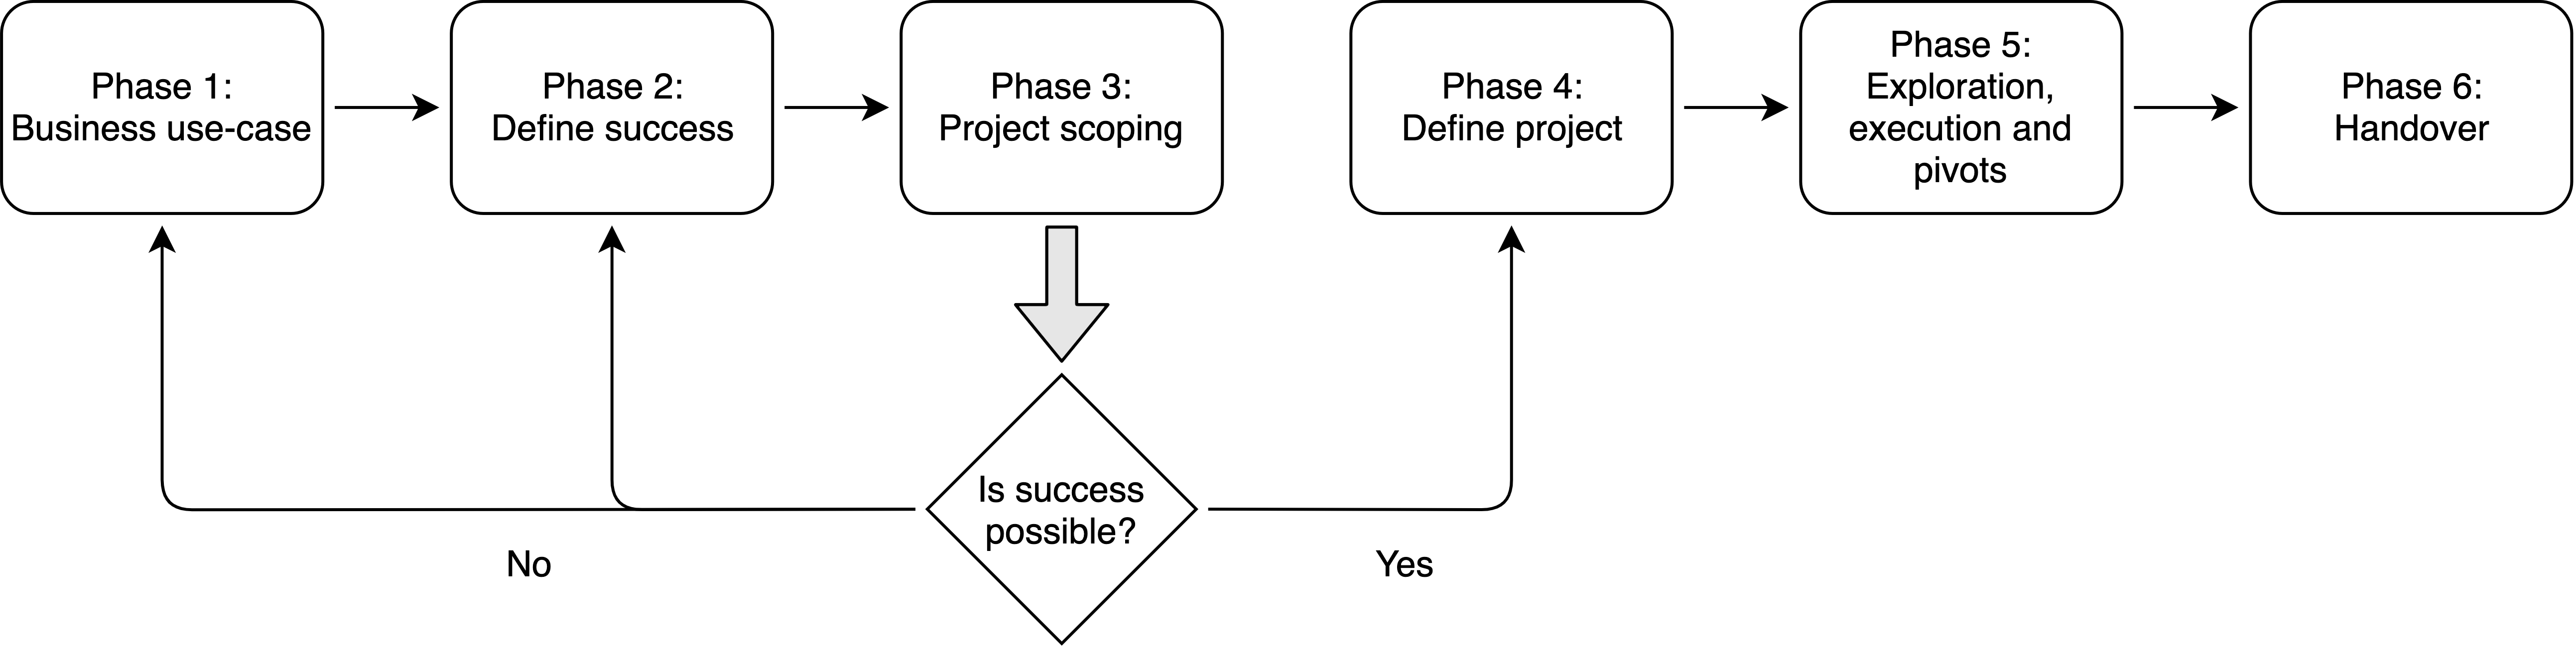
\includegraphics[width=1\linewidth]{figures/Figure_2-phases} \caption{\textbf{Six phases of a project.} When designing and delivering a project, we find it useful to break the process down into these major phases.}\label{fig:bottom-fig}
\end{figure}



\end{center}

\hypertarget{phase-1-define-the-business-casequestion}{%
\section{Phase 1: Define the business case/question}\label{phase-1-define-the-business-casequestion}}

\hypertarget{find-the-business-case}{%
\subsection{Find the business case}\label{find-the-business-case}}

You may find that your client already has a clear idea of possible projects. If that's the case, then we encourage you to go through each and view them through the lens of the contextual understandings identified above. If your client does not have preconceived ideas about possible projects, then you might want to view this conversation as a brainstorming session.

Questions that can help to drive the conversation can include:

\begin{itemize}
\tightlist
\item
  Do you have any ideas already that you would like to consider?
\item
  If you could improve three aspects of your business, what would they be?
\item
  Do you have a concrete objective or are you trying to implement a more general innovation in your business?
\end{itemize}

As you drill down into specific project ideas, you should consider the practical aspects of delivering the project. For example, we often ask our clients to describe to us what a successful outcome would be, what would be acceptable and what would be outstanding. These questions can be in terms of concrete modelling metrics (such as accuracy, precision, recall, etc) or terms of business value (for instance, to save at least £10,000 in lost annual revenue from customer churn). Asking for concrete examples of outcomes can help you to get a sense of your client's expectations and will allow you to manage these in advance.

You will also want to understand what your client will need in terms of deliverables, by which we mean the tangible \emph{thing} that is delivered at the end of the project. This could include things such as reports, presentations or a code-base, but often also includes a fully-functional software package, a deployed model or API.

Similarly, it can be useful to assess your client's appetite for risk by asking questions such as, ``If our best model is only correct half the time, would that be acceptable?''

\hypertarget{define-the-business-case}{%
\subsection{Define the business case}\label{define-the-business-case}}

As with any scientific experiment, a critical first step in designing a data science project is to define the question and to phrase a hypothesis. In other words, it is vital that all parties, including the data scientists and the stakeholders, agree on the project's goals. While a project brief can help identify important aspects of the work, in our experience the best results come from face-to-face conversations. Do not restrict this to a single person, but rather make every effort to talk to every stakeholder who may be involved in the project.

With a client I once worked with, the main stakeholder turned out to be the CFO (Chief Financial Officer). Although he was in no way involved in the project he was the one who created the budget required for the innovation. When asking the other stakeholders about the budget and requirements his name came up and we decided to include him in the next meeting. At the next meeting, we discussed the scope and even expanded the scope and budget as we were finally talking to the main stakeholder. If however this interaction had not occurred, the project would have taken a completely different direction.

When talking to the the different stakeholders, ask yourself whether a clear vision forms from these conversations and, more importantly, whether the different visions from the different stakeholders are aligned. When they are not aligned, it is your responsibility to align them. Find the middle ground and make compromises between the different parties. There is never going to be an infinite budget so you will always need to compromise somewhere.

In a related way, it is important to recognise that different stakeholders will almost always come from different backgrounds and have different preconceptions that can influence the way they perceive business problems and potential solutions. As a consultant, you want to take these different points of view into account, and you may even find that you have to defend your point of view as well.

A common pre-conception is that artificial intelligence is complicated and cannot be understood. It is often treated as a black box with a magical outcome. Developers who use machine learning libraries without fully understanding these often create or support this preconception. This viewpoint, however, originates from a lack of knowledge. Most machine learning libraries are open source and a skilled data scientist will be able to dig into their models and alter or understand the results it produces.

Machine learning models at the core are mathematical models, data is manipulated through a series of mathematical operations. These operations are not random but should be well chosen to produce favourable results. Understanding this process lets you understand the limitations and the overall behaviour of the model. Once this is properly understood, one can make deliberate changes that improve the model overall, remove bias or simply deal better with outliers that had been neglected previously.

\begin{infobox}

\textbf{What is open source}

Open Source is any computer software that is distributed with its source code available for modification. That means it usually includes a license for programmers to change the software in any way they choose: They can fix bugs, improve functions, or adapt the software to suit their own needs.

\end{infobox}

As a side note be aware when choosing your machine learning toolkit. When using closed and proprietary systems like those provided by IBM, Google and Amazon, be aware that data scientists will lose visibility and the ability to understand the system fully.

When talking to your stakeholders, do not be shy: understanding what the different stakeholders know and value is essential to forming a plan and ensuring that everyone is ``on the same page.''

In this phase, you should be focusing on the contextual and business levels. As a data scientist, it is your responsibility to make sure you and your teammates have thought carefully about what will bring value to the business and whether or not the candidate project aligns with the business strategy long-term. Fully consider how the business will change over time and what will be needed to keep this new part of the system up to date so that it can remain relevant.

Systems are in development constantly, the more you learn about the overall product and future of the product through the roadmap, the more you can use this knowledge to make your part of the system more robust. Is one of the data sources being replaced by a richer data source in future? If so how can you build your system so that this can be easily incorporated in your model when this data arrives and how will your models deal with the inconsistency in your old and new data? Writing a recommendation engine for an e-commerce site can be straightforward but how can your model use the clickstream data that will be collected in the future if you do not have this data now? These scenarios, as well as many others, can lead to technical debt in a data science pipeline. While a comprehensive review of how to minimise technical debt is beyond the scope of this article, we recommend \href{https://www.amazon.co.uk/Managing-Technical-Debt-Development-Engineering/dp/013564593X/ref=sr_1_1?dchild=1\&keywords=managing+technical+debt\&qid=1595912830\&sr=8-1}{Managing Technical Debt}.

\hypertarget{phase-2-define-success.}{%
\section{Phase 2: Define success.}\label{phase-2-define-success.}}

After going through Phase 1, you and your client/manager should have a clear picture of what the main objectives of the project are. Now it's time to narrow in on some details. In this phase, you will address specific requirements to make sure that you and your client/manager agree on what a successful outcome will look like in concrete terms.

As part of defining success, it will be essential to map out the business and identify the various people and departments involved in the project. You may find that each stakeholder has a different picture of what a successful outcome looks like, so you must be sure to address these differences and align them as best you can. Project planning is all about negotiation, negotiate with the different parties until you get everybody to align to the same vision. Note that without alignment you can't proceed, if you do proceed by choosing to align to the main stakeholder, the other stakeholders will be hostile towards you and the project. If there is a conflict you can't possibly resolve, take this up with the most senior person so that they can pull rank and force alignment this way.

When fleshing out your feature list, It can be useful to make two different lists, one with the must-have requirements and one with the nice to have. You can then move different items between the lists when talking to the different stakeholders. When everybody agrees with the final list, you have an agreement and you can focus on implementing the essential requirements while possibly leaving space for some of the less important requirements.

At this point, it is also important to think about the bigger picture and what the end product will look like and how this can be achieved. For example, if the end goal is to have a feature in production, then now is the time to figure out how the deployment process works. Consider questions such as who has access to this process? Do you need to get engineers involved and what does their availability look like?

In order to be successful, it is essential to consider how we will measure success. Refer back to Chapter \ref{levels} and define success on the four different levels: the project process, product, business and contextual level. For project and process level success we will need to define a metric that accurately reflects the problem that we are trying to solve. This metric is often tied to a business objective. For instance, if we are automatically classifying incoming emails then success could be defined as a system that classifies 95\% of all incoming email correctly. In this case, you should also define `correctly'. Here, `correct' would be that the classification algorithm has the same outcome as a skilled employee. The exact number you choose will be a tradeoff between accuracy and the budget/time spent.

Most companies will already be working with a way to keep track of and define success for it's varying departments, this is often framed as Key Performance Indicators.

\hypertarget{KPIs}{%
\subsection{Key Performance Indicators (KPI)}\label{KPIs}}

\begin{infobox}

\textbf{Definition}

A Key Performance Indicator is a measurable value that demonstrates how effectively a company is achieving key business objectives. Organizations use KPIs at multiple levels to evaluate their success at reaching targets. High-level KPIs may focus on the overall performance of the business, while low-level KPIs may focus on processes in departments such as sales, marketing, HR, support and others.

\end{infobox}

KPIs are widely used within organisations to measure business objectives. To find KPIs that are relevant to your project you should be able to answer the following questions:

\begin{itemize}
\tightlist
\item
  What is your desired outcome?
\item
  Why does this outcome matter?
\item
  How are you going to measure progress?
\item
  How can you influence the outcome?
\item
  Who is responsible for the business outcome?
\item
  How will you know you've achieved your outcome?
\item
  How often will you review progress towards the outcome?
\end{itemize}

One way to evaluate the relevance of a performance indicator is to use \href{http://en.wikipedia.org/wiki/SMART_criteria}{the SMART criteria}. The letters are typically taken to stand for \textbf{Specific, Measurable, Attainable, Relevant, Time-bound}. In other words:

\begin{itemize}
\tightlist
\item
  Is your objective \textbf{Specific}?
\item
  Can you \textbf{Measure} progress towards that goal?
\item
  Is the goal realistically \textbf{Attainable}?
\item
  How \textbf{Relevant} is the goal for your organization?
\item
  What is the \textbf{Time-frame} for achieving this goal?
\end{itemize}

\hypertarget{feasibility-study}{%
\subsection{Feasibility Study}\label{feasibility-study}}

A feasibility study aims to objectively and rationally uncover the strengths and weaknesses of a project in order to assess the likelihood of its success. In its simplest terms, the two criteria to judge feasibility are cost required and value to be attained. For data science projects we tend to focus on technical, economic, legal, operational and scheduling feasibilities.

\hypertarget{technical-feasibility}{%
\subsubsection{Technical Feasibility}\label{technical-feasibility}}

The technical feasibility assessment is focused on gaining an understanding of the present technical resources of the organization and their applicability to the expected needs of the proposed system. It is an evaluation of the hardware, software and technology required to meet the needs of the proposed system.

This assessment is based on an outline design of system requirements, to determine whether the company has the technical expertise to handle completion of the project. When writing a feasibility report, the following should be taken into consideration:

\begin{itemize}
\tightlist
\item
  A brief description of the business to assess more possible factors which could affect the study
\item
  The part of the business being examined
\item
  The human and economic factor
\item
  The possible solutions to the problem
\item
  Methods of producing the solution
\item
  Detailed project requirements
\end{itemize}

This detailed report should stipulate if a project is technically feasible. There are many reasons why projects aren't technically feasible and it could be as complex as the requirements aren't simultaneously achievable or the company does not have the know-how to build and maintain the proposed system even if it is technically possible to do so.

\hypertarget{economic-feasibility}{%
\subsubsection{Economic Feasibility}\label{economic-feasibility}}

An economic feasibility study typically involves a cost/benefits analysis of the project, helping organizations determine the viability, cost, and benefits associated with a project before financial resources are allocated. It also
serves as an independent project assessment and enhances project
credibility---helping decision-makers determine the positive economic benefits to the organization that the proposed project will provide.

\hypertarget{legal-feasibility}{%
\subsubsection{Legal Feasibility}\label{legal-feasibility}}

The legal feasibility assessment investigates whether any aspect of the proposed project conflicts with legal requirements like zoning laws, data protection acts or social media laws. Let's say an organization wants to store customer information for the use in a recommendation engine on its e-commerce site. A feasibility study might reveal that the laws governing this data differ depending on where the customer is geographically located. Therefore, simply storing this data isn't possible and a more in-depth analysis of the law needs to be made. Different data will need to be stored for different customers. This might mean that the recommendation engine isn't feasible for the organisation right now as this would add extra costs and technical difficulty.

\hypertarget{operational-feasibility}{%
\subsubsection{Operational Feasibility}\label{operational-feasibility}}

The operational feasibility study involves undertaking a study to analyze and determine whether---and how well---the organization's needs can be met by completing the project. Operational feasibility studies also analyze how a project plan satisfies the requirements identified in the requirements analysis phase of system development.

To ensure success, the desired operational outcomes must be imparted during design and development. These include such design-dependent parameters as reliability, maintainability, supportability, usability, producibility, disposability, sustainability, affordability and others. These parameters are required to be considered at the early stages of the design if desired operational behaviours are to be realised. System design and development requires appropriate and timely application of engineering and management efforts to meet the previously mentioned parameters. A system may serve its intended purpose most effectively when its technical and operating characteristics are engineered into the design. Therefore, operational feasibility is a critical aspect of systems engineering that needs to be an integral part of the early design phases

\hypertarget{scheduling-feasibility}{%
\subsubsection{Scheduling Feasibility}\label{scheduling-feasibility}}

The scheduling feasibility assessment is the most important study for the project's success; after all, a project that is delivered too late to be useful is an automatic failure. In this study, we estimate how long the system will take to develop, and if it can be completed in the given time. Time feasibility is a measure of how reasonable the project timetable is. Given our technical expertise, are the project deadlines reasonable? Some projects are initiated with specific deadlines. It is necessary to determine whether the deadlines are mandatory or desirable.

\hypertarget{phase-3-scoping}{%
\section{Phase 3: Scoping}\label{phase-3-scoping}}

This is the phase where we start to explore the supporting data and test some of our hypotheses and assumptions. Note that the goal of this phase is not to create a proof-of-concept; this phase has no concrete deliverables and is more open-ended. Rather this phase is aimed at understanding the size, structure and complexity of the supporting data and to generate a clearer understanding of the problem and what a solution could look like.

Usually this phase starts with a data exploration, during which you should be asking questions such as:

\begin{itemize}
\tightlist
\item
  Are the data in a clean usable format?
\item
  If not what manual/automated effort would be required to get the data in a usable format?
\item
  How complex are the transformations required?
\end{itemize}

Once you have the data in a usable format, you should ask standard EDA (exploratory data analysis) questions: What abnormalities does the data set have? What do the distributions look like? Is the dataset uniformly distributed or is it sparse and does it have a lot of outliers? How are missing values recorded? How many missing values are there? Are there any unusual entries that require explanation?

\begin{infobox}

\textbf{Data access and security}

Getting access to data can often be a challenge due to security policies that may be in place. This is especially common in financial services, but is certainly not limited to this industry. There are many ways of making data access secure so you may have to work with the data administrators to work out a safe and secure plan that works for them. We have each had to endure inconveniences to access data, such as sitting in data-secure rooms with no internet access, having encrypted laptops sent to us to use for our work or having had to access data via VPNs and cloud-based servers that restricted access based on multi-factor authentication. For some industries, we have even had to go through extensive background checks. There are often quite a few hurdles to jump through when it comes to data security so we recommend discussing this with your client early in order to get these hurdles out of the way.

\end{infobox}

What defines clean data can vary greatly across professions and industries. For some people, hundreds of differently structured excel files that are human-readable would be considered clean data, while for data scientists this would be a nightmare, requiring a substantial investment to merge all of the files for them to be analysed as a coherent whole. Databases or data warehouses, in contrast, tend not to suffer from such problems of \emph{data structure}. However, even well-structured data can require substantial cleaning. For example the dataset could contain duplicate entries, missing values or inconsistently-recorded measurements, to name but a few potential data cleaniness problems. While exploring and working with a poorly-structured or unclean dataset may be agonising, knowing the state of the data that you will use for the project is critical in order to accurately appreciate the scale of the prospective project. Unexpected data cleaning can take weeks and will invariably cause delays to your project, so this insight will allow you to budget appropriately when creating your project plan.

The next step is reducing some of the uncertainty and risk by carrying out hypothesis testing. What do we mean by that? In one way, we mean statistical hypothesis testing in the truest sense of the word: formulating null and alternative hypotheses and apply appropriate statistical tests to see how well the evidence supports them. However, we also mean testing more general ideas about the data, usually based on anecdotal evidence or domain experience from those who know the business the best. For example, your client may be confident that sales are highest on Fridays -- use that as the basis for an experiment in your EDA and see if the data really do support that notion. Often with such assumptions, the data will indeed confirm what your client \emph{knows} (or, more accurately, \emph{thinks they know}) about the data. But sometimes those assumptions are wrong, and you are unable to find support for the assumption \emph{in the data you have}.

It is important to note here that hypothesis tests that fail to support your clients assumptions do not necessarily mean that those assumptions are false. We emphasised the words ``in the data you have'' in the preceding paragarph for a reason: your data may not be representative of reality. This touches on a fundamental notion in data science -- that data is not the same as ground truth. Data are artefacts and are affected by biases in collection methodology, collection strategy, storage, aggregation and interpretation. In short, the data that comes to you has been affected by the many design choices that were made by others -- choices about every step on the journey between the real world and the number you see in front of you on your computer. No dataset is ever completely unbiased. In an ideal world, you (the data scientist) would have a say in how data are collected and curated. In reality this almost never happens, leaving you to work with data that has been affected by the choices of others.

During this phase of the project, you will want to validate some of the foundational assumptions upon which your project will be based. Our advice is to do this in as scientific a way as possible so that you can be as accurate as possible about what will be involved to deliver the project objectives.

Almost always, a data science project
All We are dealing with a scientific question which rely on several assumptions, so the more we can validate these assumptions the better we will be able to predict the eventual outcome of the overall project. One common assumption is that having sufficient data will automatically lead to predictive power. The size of your dataset sadly doesn't indicate how good the individual features are at predicting a specific behaviour. It is also good to remember that \href{https://medium.com/@angebassa/data-alone-isnt-ground-truth-9e733079dfd4}{data alone isn't ground truth}.

It is essential that this phase is time-boxed, for example, a 2-week POC (Proof of Concept) for research projects or just a couple of hours to look through data. This allows the team to focus their efforts on the most pressing concerns without starting to implement the entire project. \textbf{The goal is not to get started but rather to reduce risk and explore possible solutions.} In software engineering, this is often done in the form of a design sprint. In data science, we can also work in sprints but the process is slightly different as we need to validate a hypothesis, and so the process is far more scientific. Doing this work beforehand helps us drastically reduce uncertainties and even guarantees that projects that are doomed to fail don't even get started. If at this stage we discover there is insufficient or insignificant data to reach the goal then we can go back and collect more data and delay the project until its goals are achievable.

The reader might think that doing this phase is hindering the project -- delaying it from really getting started and providing little in the way of tangible outcomes. In our experience, this is untrue: when we scope out a project we can more accurately predict what the outcome will be and what resources are needed to achieve the end goal. This translates into less risk for clients and data scientists alike. Being able to quickly demonstrate progress or build a basic proof-of-concept reassures all stakeholders that the project will be successful. This also stops us from adding large margins to project proposals to combat the uncertainty and ultimately delivers project proposals that better reflect reality, which is better for all stakeholders involved. We have personally had a 100\% success rate of winning project proposals as an independent consultant once we embarked on this stage. The reason is clear, having had time to scope out the project our proposal was more competitive as we didn't need to add large margins for project uncertainty.

\begin{infobox}

It is essential to note that general engineering projects differ from data science projects. Data science projects need to be scientifically correct and for this, you need to follow a scientific process. It is not enough to make a library call to train a model and assume it will perform a certain way just because you tested a few cases. Models you create need to be robust or you will get large varying results that cannot be explained. Making models robust to outliers is an important step in modelling. So be warned, it is not enough for somebody to have used a machine learning library in the past, they should be capable of following a scientific process required to build what is necessary for a data science project to succeed.

\end{infobox}

In this phase, it is also essential to start thinking about testing. How will you test your final solution? Can you use TDD (test-driven development)? This strategy requires you to set up extensive test cases now that you will use to validate your final solution later. Doing this will let you think through the problem more clearly and write down what criteria the result will adhere to.

The last thing to consider in this phase is that you might not get the desired outcome. It is essential that you allow the scoping project to fail if need be. At the very least you saved yourself from failing at a larger scale. Most probably you will discover shortcomings that will not allow the project to be successful. How can these issues be addressed? Can more data be collected? Can the data be enriched with another source? )r can data be cleaned even further to get a better sample? A valid outcome is to make a good recommendation as to how the project can still be successful by doing other work. For example, can clickstream data be collected from the website if there are insufficient orders to make decent recommendations for customers who have never bought an item? This would solve the cold start problem many recommendation engines face.

\hypertarget{phase-4-project-definition}{%
\section{Phase 4: Project definition}\label{phase-4-project-definition}}

In the previous scoping section we got to do some hands-on work. At this point, you have understood the business case for your project and had a look at the data that will support the work. You will also have defined what a successful outcome is, established metrics for measuring success and developed a clear understanding of the complexity of the task in front of you. The next steps are to concretely define the project, describe it in the form of a written proposal and put a price tag on it. Welcome to Phase 4: Project definition.

This is a difficult task and it comes with a large number of considerations that you need to take into account. We have, therefore, put a detailed description of how we approach this in a subsequent chapter. Here we highlight a few of those factors.

When defining your project, it's good to start with a project plan that can be broken down into milestones. Think about what the objective of each milestone is, and what deliverable will mark its completion. What skills will be needed for the work? If you are building a team, you'll want to make sure they have what's required; if you're working on your own, will you have to do any homework to ensure that you have the experience that is needed. You will have to put a price on the work and think about how the project will be managed. These items are discussed in detail in Chapter \ref{definition}.

\hypertarget{phase-5-exploration-execution-and-pivots}{%
\section{Phase 5: Exploration, execution and pivots}\label{phase-5-exploration-execution-and-pivots}}

This is probably the most exciting phase as we have come to the actual execution of the project. Firstly we will start by doing research, the research sets the groundwork for the entire project. It is here that we discover what works and what doesn't. We try different approaches, weighing the pros and cons of each before selecting a final solution.

This phase is different from the scoping done previously as now the goal is to develop and deliver on the full scope. The scoping exercise only delivered a good idea on what the solution might look like, not necessarily an optimum one. In this phase, we are looking for a solution that meets all of the requirements. To elaborate, the scoping exercise might have produced a model capable of predicting good results but not necessarily at a speed or larger scale required for production.

Once we have made these decisions and agreed on them with the client/manager we are ready to start building. If however, you do not get agreement at this point, have a longer session to flesh out any other requirements.

In this step, we go deeper into the chosen approach. Deeper may mean using all of the data instead of just a sample, improve feature engineering, improve model accuracy, do a deeper analysis or even build a viable usable product.

Throughout this process, we will evaluate our results and possibly move back to the building stage or even the research stage if we do not have adequate results. Client engagement is critical and we will include them regularly. For further details on these stages see Chapter \ref{execution}.

\hypertarget{phase-6-handover-and-knowledge-transfer-aka-finding-a-new-owner}{%
\section{Phase 6: Handover and knowledge transfer (aka finding a new owner)}\label{phase-6-handover-and-knowledge-transfer-aka-finding-a-new-owner}}

Sometimes this phase is really simple. If the deliverable was a report then nothing further needs to be done. For more complex projects this, however, can be the most difficult phase.

If you are creating a system, remember to deploy the solution according to the plan. It is often not enough to hand over source code as crucial details are often in the deployment. Does your solution scale? Make sure to stress test your application so that it doesn't crash unexpectedly.

For the long term success of any project, there must be a long term strategy in place. The software will always need to be maintained and depending on what you developed models might ingest new data and the results will slowly start to drift over time. How will the organisation deal with this? Is there a plan in place to maintain these models over time and who will do this?

\begin{infobox}

\textbf{The concept `drift' explained}

In the most challenging of data analysis applications, data evolves and must be analyzed in near real-time. Patterns and relations in such data often evolve, thus, models built for analyzing such data quickly become obsolete over time. In machine learning and data mining, this phenomenon is referred to as drift.

To combat drift, a model should be thoroughly analysed and a decision needs to be made on how frequently a model should be re-trained in order to remain relevant.

\end{infobox}

Oftentimes those that develop a system are not those that need to maintain it long term. This by itself might cause many issues but to make sure this goes as smoothly as possible be sure to write clear concise code, following coding standards, writing detailed documentation and having decent test coverage. Regarding documentation, it is best practice to write your comments and documentation alongside the actual code. Doing this will mean your documentation is more likely to stay up to date. If documentation is in a different location than the code, then a developer making changes, would also need to remember to update the documentation.

Many great tools can generate beautiful looking documentation from comments added in your code. For python, we can highly recommend \href{https://www.sphinx-doc.org/en/master/}{Sphynx} as it is widely used and gives you loads of great styles to choose from.
Regarding proper coding style, we recommend you follow \href{https://www.python.org/dev/peps/pep-0008/}{PEP8} for python and for R, the \href{http://adv-r.had.co.nz/Style.html}{R style guide}. We recommend you install a linter into your text editor so that your code will be constantly checked against these coding standards. Coding standards make your code far more readable so it is recommended to adhere to them as much as possible, We also find it useful to use a formatter, for python we use \href{https://github.com/psf/black}{Black}. This will automatically format your python code to meet the PEP8 guidelines. You will never need to worry about code formatting again as a formatter can automatically add the correct spacing, line breaks and other coding standards. It is, however, important to note that once you use a formatter, you can't realistically override the formatting and you will need to accept some style changes as is. Every time you run your formatter these changes will be undone so there is no point sticking to your preferred format.

When you reach the end of your project, find the person responsible for maintaining the system and run through how it works. Do a complete handover running through both the code and the documentation, adding comments and notes to clarify points that are not clear to the person you are handing over to.

If handover to an actual person is not possible for whatever reason, eg. if a permanent data scientist is not yet hired, then make sure you make your documentation as clear as possible. Do not leave it to chance and write it as if you are writing for a very junior person. More documentation is recommended in these cases.

Make sure the test cases are understood and implemented in such a way that they are run regularly. There are plenty of continuous integration tools that do this for you. This will stop any performance altering changes from taking place. To avoid the negative consequences of model drift, recalculate the model performance on new data regularly.

\hypertarget{chapter-summary}{%
\section{Chapter summary}\label{chapter-summary}}

In this chapter, we have given you a lot of information about how we approach the projects that we design and execute. We hope that you find our suggestions useful. Naturally, projects come in different sizes and scopes, and whether or not all of these phases are appropriate for a given project depends on many factors.

While we have presented project evaluation and project phases as different concepts, in actuality they go hand-in-hand. We encourage you to think about the levels of project evaluation as you go through the phases of project design. As we saw in Chapter \ref{levels}, the levels of project evaluation are hierarchical. They also have a temporal component, by which mean that one should think about the higher levels during the earlier phases of a project when the business case is being discussed. The lower levels, such as the \emph{project process} phase come more into consideration during the later phases of scoping, execution and handover. To illustrate this point, we have combined the earlier two figures into the figure before.



\begin{center}

\begin{figure}
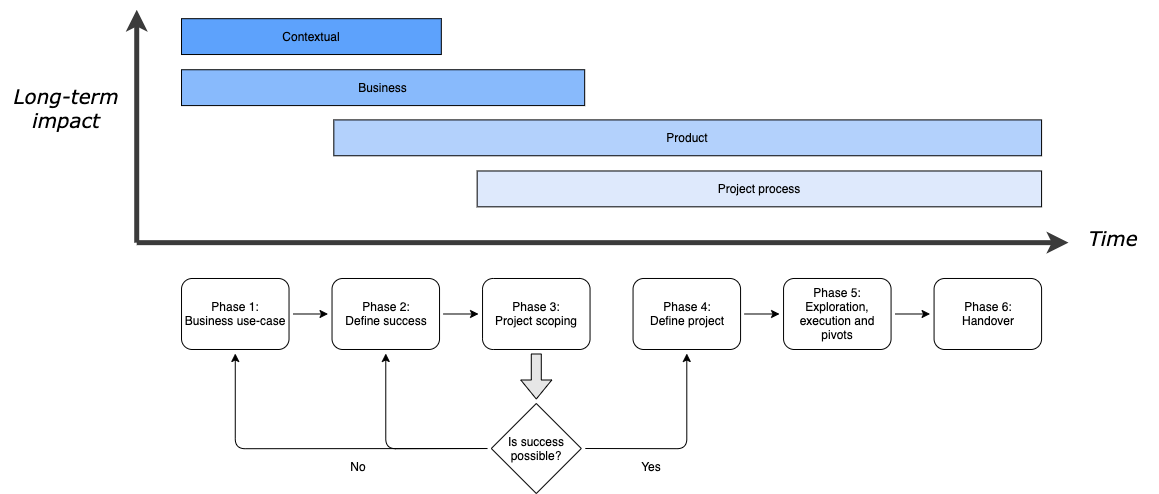
\includegraphics[width=1\linewidth]{figures/Framework phases} \caption{Combined project evaluation and phases}\label{fig:full-figure}
\end{figure}

\end{center}

\hypertarget{definition}{%
\chapter{Deep dive into Phase 4 -- project definition}\label{definition}}

If you have followed the steps outlined in phases 1-3, you will have now determined that the project is viable. You will have confirmed that, in principle, the project makes contextual sense and that it is likely to bring value to your stakeholder, and you are now ready to think in terms of the specifics about how you will deliver the work. Congratulations! This represents a major crossroads for any project, and you should be proud of yourself for having had the discipline to work through Phases 1 -- 3 carefully. Now you are ready to start your project in earnest!

But hold on! Before you start writing code and delving into the work, you must plan the project -- that is what Phase 4 is about. This is the design phase, where you lay out in detail the approach you will take, the steps that will be included and the resources that will be required. We often hear people say things such as, ``Data science is research\ldots how can I say how long it will take if I don't know what I'm going to find?'' This is a valid concern -- in an ideal world, you would have all the time and money you need. Sadly, this is an example of the difference between the ideal world and reality: if you are working with a client/manager, you will need to inform that client/manager what will be required in terms of time and money. Can you be certain that your estimations are sufficient? No.~But you can make reasonable estimations with the information you have, and this is where the art of project design comes in.

It isn't always possible to have a robust plan but having a flawed plan is always better than none at all. A plan helps break down the task into smaller more manageable tasks that can be done and progress can be shown. It also helps everyone understand the deliverables and the course of action. Changing a plan can always be done but operating without a plan will always be slower than without one.

This phase uses a different type of thinking than is normally found in scientific research. While research generally uses deductive (the reasoning of logic) and inductive (the reasoning of forming general rules from observations) reasoning, the synthesis required for design thinking uses intuition, or more accurately, abductive reasoning -- the reasoning of developing one of several possible solutions for a problem. More specifically it is seeking the simplest solution to a problem without any formal validation. For a more detailed explanation of how designers think, we recommend the book Design Thinking by Nigel Cross. For the purposes of this writing, what is important is to understand that this relates to the process of identifying a set of required functionalities or purposes and crafting a solution that satisfies those purposes.

\begin{infobox}

\textbf{What is abductive reasoning?}

Abductive reasoning starts with an observation or set of observations and then seeks to find the simplest and most likely conclusion from the observations. This process, unlike deductive reasoning, yields a plausible conclusion but does not positively verify it. Abductive conclusions are thus qualified as having a remnant of uncertainty or doubt, which is expressed in terms such as ``best available'' or ``most likely''.

\end{infobox}

For many, project design is difficult, ambiguous, stressful and downright unpleasant. Indeed, this phase requires you to commit to delivering a given bit of work in exchange for a certain budget, and you want to get it right -- who wouldn't find that responsibility stressful? You inherently can't know exactly what it will take to deliver a successful outcome because that insight only really comes from the work itself. But if you have done a good job of scoping the project in Phases 2 and 3, then you should have a fairly good idea of the complexity of the task in front of you.

\hypertarget{developing-a-project-plan}{%
\section{Developing a project plan}\label{developing-a-project-plan}}

We suggest you begin by thinking at a high level. Where are you starting from, where do you want to be when the project is completed, and what are the logical steps you need to take to get there? What are the functionalities that are required, and which ones would be nice to have but are not critical? What are the novel concepts and approaches you will have to develop? Are there logical intermediate steps along the way? Does something depend on something else being completed first?

In most cases, we break a project down into stages with aims and milestones. We find it useful to clearly define what work will be carried out in each stage and what will be delivered at the end of it. Sometimes a ``deliverable'' is merely a short report, a small presentation or a conversation with your client/manager. In other cases, it can be a piece of software or a tangible functionality that can be demonstrated. Exactly what the deliverable at the end of each milestone looks like is project-dependent.

In the best cases, each milestone in itself is a valuable step forward for the stakeholder. This de-risks the entire project. For example, a project may be aimed at building an interactive data analytics dashboard with four milestones along the way. Milestone 1 may be an in-depth exploratory analysis that can yield important insights about the data. If their project were to end there, the work would still have brought value. While this is not always possible, we suggest you keep this in mind as something to aim for when crafting your project timeline and stages/milestones.

Throughout this process, it can be useful to consider pivot points or alternative outcomes. For example, many projects have milestones that are inherent points for decision-making. If that is the case for your project, be sure to communicate that clearly in your project plan. When making these decisions, try to balance flexibility and open-mindedness with a clear view of business value.

In the earlier scoping phases, you will have determined what the requirements of the project are in terms of outcomes and deliverables. If these include data products that require engineering or deployment (as opposed to projects primarily focused on the generation of insights and models), you will need to include corresponding milestones. Data cleaning, code refactoring, optimisation and productization can be time-consuming, as can deployment of your product and the development of sound ETL pipelines -- be sure to budget for these in your project plan and think carefully about what a sensible development plan looks like.

\hypertarget{what-skillsexpertise-is-required}{%
\section{What skills/expertise is required?}\label{what-skillsexpertise-is-required}}

As you plan your project, the required technical and non-technical skills should start to become clear. Many skills can be thought of as more general, such as coding, machine learning or results orientated. Others are more specialised, such as natural language processing or graph theory. And yet other skills are harder to come by, the domain-specific expertise. Ensuring you have the industry-specific experience to deliver the project or make sure that you have willing sponsors within the company who will set aside time to work with you on understanding any industry quirks and nuances.

Your approach to meeting the skills required for a project is, of course, dependent upon the composition of your team. If you are designing a project that you will work on individually, then it is up to you to make sure you have the skills required in your repertoire. If you don't, you may need to consider bringing in outside help or budgeting for the time it will take to level-up your shortfall. Often projects are designed for teams of data scientists, in which case you will want to make sure that the skills required are matched collectively by the team. Data Science as software development is a team sport.

\begin{quote}
``If you want to go fast, go alone. If you want to go far, go together.'' -- African Proverb
\end{quote}

\hypertarget{how-much-will-it-cost}{%
\section{How much will it cost?}\label{how-much-will-it-cost}}

You will almost certainly have to put a price tag on your project. For us, this is essentially a calculation based on how long we think the project will take and the billing rate for the staff. Junior/mid-level/senior data scientists all have different rates to consider in this calculation. The staff billing rate is normally constant, so we tend to focus primarily on the duration of the project.

As discussed above, getting this right can be difficult. If your estimate is too low you may not have the time needed to complete the work; if it's too high, you risk losing the contract. The latter case is especially relevant if you are competing against other providers, for example in the case of a proposal written in response to an RFP (request for proposals). For other projects, the cost factor might not be important at all as employee projects often overrun without any negative consequences. For those to whom the cost factor is important, we don't have a magic formula that tells how to strike the right middle ground. What we can do is highlight some considerations that we find helpful in the process and offer our reassurance that it gets easier to make this judgement as you become more experienced.

Breaking the project into milestones as described above can help: it's easier to estimate the time required for smaller tasks than for larger ones. Understanding the supporting data will also help, which is a major reason for the scoping work described in Phase 3. This is also a place where having a solid network to turn to for advice might be very useful. At Pivigo, for example, our data team discusses each project plan that is being written to get as many different points of view as possible. If you have access to a network of peers, going through such a sense-check can be a very valuable process. Experience is key, look at different case studies or ask colleagues about similar projects and how long it took to do those.

It can help to anticipate places where the work is at a higher risk for delays. For example, you may have made assumptions about the data structure based on your scoping work, only to find out that some of these assumptions are not correct. The data coming in may have changed in structure or location, or unanticipated factors may have worked to introduce more missing values than you expected. You can't anticipate every possible roadblock, but if you can identify places where your progress is most vulnerable to problems, you can make a conservative estimate.

It is also useful to consider the business when budgeting for a project. Have you worked with this company or person before? If you have, and if the project was successful, you probably have earned a degree of trust that can go a long way in convincing them that your proposal is reasonable. In contrast, if the business is new to data science, or new to you, you have yet to earn their trust and may want to be more cautious in how you cost your project. Similarly, if you feel that your client/manager has the potential for being demanding and hard to please, it may be a good idea to err on the side of caution by budgeting a bit generously. In these cases, the costs of underestimating the required time are high.

On the other hand, if the project is exploratory, if your client/manager is just looking to see the ``art of the possible'' or if your project is restricted to creating insights, you may feel a bit braver and choose a slightly lower budget: the costs of underestimating the time required are lower. Or, to think of it in another way, even if you only accomplish 95\% of what you would have liked, that is still very valuable for the business.

\begin{smaller}

\begin{longtable}[]{@{}lll@{}}
\toprule
\begin{minipage}[b]{0.22\columnwidth}\raggedright
Pricing\strut
\end{minipage} & \begin{minipage}[b]{0.35\columnwidth}\raggedright
Potential\_benefits\strut
\end{minipage} & \begin{minipage}[b]{0.35\columnwidth}\raggedright
Risks\strut
\end{minipage}\tabularnewline
\midrule
\endhead
\begin{minipage}[t]{0.22\columnwidth}\raggedright
Under-budgeting\strut
\end{minipage} & \begin{minipage}[t]{0.35\columnwidth}\raggedright
\begin{itemize}
\tightlist
\item
  Your proposal may be
  more attractive to the
  stakeholders.
\item
  The potential to show
  your client/manager good
  value-for-money
\item
  Get a ``foot in the
  door''/opportunity to
  prove yourself
\end{itemize}\strut
\end{minipage} & \begin{minipage}[t]{0.35\columnwidth}\raggedright
\begin{itemize}
\tightlist
\item
  Your client/manager may
  be sceptical that you can
  deliver
\item
  You may not be able to
  deliver
\item
  You are vulnerable to
  expected problems
\item
  Setting the
  expectation too low for
  the follow on work
  (assuming you get it)
\end{itemize}\strut
\end{minipage}\tabularnewline
\begin{minipage}[t]{0.22\columnwidth}\raggedright
Over-budgeting\strut
\end{minipage} & \begin{minipage}[t]{0.35\columnwidth}\raggedright
\begin{itemize}
\tightlist
\item
  Extra time padding can
  give you a greater chance
  of success
\item
  Greater chance of
  overdelivering and
  delighting the
  client/manager
\item
  Greater chance of more
  work, due to happy
  client/manager
\end{itemize}\strut
\end{minipage} & \begin{minipage}[t]{0.35\columnwidth}\raggedright
\begin{itemize}
\tightlist
\item
  Your price may be too
  high/losing the work
\end{itemize}\strut
\end{minipage}\tabularnewline
\bottomrule
\end{longtable}

\end{smaller}

It's also useful to think about aspects of the project that are ``must-haves'' versus those that are ``nice-to-haves''. At the very least, your budget should give you enough time to safely deliver the must-haves. Taking a slightly more risky approach to the nice-to-haves may be more aligned with your client's or manager's appetite. This is especially true if your client/manager is on a tight budget. In such cases, an approach we often take is to write a proposal with several costs: a cost for the essential (must-have) work and additional add-on costs for the nice-to-have bits. We find this resonates with clients/managers who are nervous about spending a lot of money on a project that has yet to show good ROI (return-on-investment). We also recommend treating your proposal as a step in a back-and-forth conversation with the client/manager. Invite the client/manager to comment on the content and the plan, and be open to the possibility of changing the plan if the client/manager is not comfortable with the initial version. While you may not be willing to make sacrifices in your rate (and generally you should not be), you can adjust the scope of the project to better align with your client's/manager's needs, wishes, concerns and budget. This will not only help you to find the right balance for your client/manager, but it will also help to build trust with your client/manager in the fact that you are trying to work with them to produce something that is useful and has good value-for-money.

We also encourage you to mention any other costs that the client/manager may incur. For instance, if your work requires the use of a virtual machine or the creation of a database that will be hosted on the cloud, these are costs that the client/manager will want to know about. Hosting your solution can also bring with it security concerns and other maintenance costs or complications. Be sure to be as thorough as possible. This will help your client/manager to understand the total expense of the project. It will also help in your efforts to build up a trusting relationship with your client/manager. Or, to put it another way, surprising your client/manager with unexpected expenses can undermine the trust that you are striving to build. In short, view your work with your client/manager as a relationship that has to be built and nurtured, and do your best to approach it with empathy for all the people who are involved.

\hypertarget{how-will-you-manage-the-project}{%
\section{How will you manage the project?}\label{how-will-you-manage-the-project}}

At this point, you have a project plan and you have accounted for the technical skills that will be needed to bring it to fruition. However, a final consideration is still outstanding: how will you manage the project?

As above, if you are working on a project independently, then this is probably a fairly easy question to answer. If you are designing the project for a team, then planning for the project's management will be critically important. Either way, we suggest that you take some time to consider exactly how you will work and how you will interact with your client/manager.

Project management is a large field -- we cannot give it justice in this small section. When done well, a project flows smoothly and has a clear road-map and an efficient system for sharing the workload. Everyone is happy with the work and they all feel like they are contributing towards a common goal. When done poorly or not at all, a project can stagnate and become aimless, deadlines are frequently missed and the project outcomes may not align with the project goals. Good project management cannot turn every project into a masterpiece, but it can go a long way in keeping a project on-track, focused and successful.

For some teams, a scrum approach can be useful, although you should bear in mind that this is designed for software development and there do exist significant differences between this field and that of data science. In our work, we tend to adopt an agile methodology (Scrum or Kanban), in which we work in discrete sprints and organise our tasks in the form of discrete issues. Other approaches also exist, such as the more traditional waterfall model. Tools such as Kanban boards and Gantt charts can be very helpful in planning out your project and breaking down the major phases of the project into tangible, bite-sized pieces. Even if you are a team of one, we have found that the formality of organising our work in this way can be very helpful in keeping the focus on project priorities.

In addition to planning out how you will work and communicate with your team, you should also make a plan for how you will interact with your client/manager. You should consider how you will communicate with your client/manager on a day-to-day basis (we have found Slack to be very useful) as well as how and when you will give progress reports and project updates.

We also encourage you to think about how you intend to structure your codebase. We generally use Git and GitHub for version control and code sharing, and we would encourage you to build your repository's directory structure before any code is added. We highly recommend the \href{https://github.com/cookiecutter/cookiecutter}{``cookiecutter'' family of project templates} and have found the \href{http://drivendata.github.io/cookiecutter-data-science/}{Python-based data science template} to be a good fit for most of our Python-based projects. It includes a guide to best practices for directory structure and naming conventions and contains a built-in make functionality that can be useful for managing the steps required to build the requisite datasets and functions for your project. For R-based projects, one option is the \href{http://projecttemplate.net/}{ProjectTemplate}, although others also exist. At the minimum, we encourage you to work within the \href{https://support.rstudio.com/hc/en-us/articles/200526207-Using-Projects}{framework of an R Project}.

\hypertarget{check-back-on-the-four-levels-and-evaluate-the-plan-in-the-context-of-each.}{%
\section{Check back on the four levels and evaluate the plan in the context of each.}\label{check-back-on-the-four-levels-and-evaluate-the-plan-in-the-context-of-each.}}

If you have followed the steps above, you will now have defined your project. You will have a project plan that includes milestones, a timeline, potential pivot points and clearly-defined deliverables. You will have determined the composition of the team needed to execute the project and have thought about how the team will work together and liaise with the client/manager. You will have also created a budget for the project based on the time required, cost of staff and any other costs required. You probably can't wait to send your proposed plan off to the client/manager and get to work!

But before you do, we encourage you to look back at the four levels of project evaluation outlined previously. Think about the business case and the larger context of the project in relation to the business strategy, and ask yourself if what you have planned will be impactful. If you are not convinced that it will be, you may need to reconsider your plan.

As a parting piece of advice, we suggest that you take the time to make a shortlist of ways that the project is likely to be impactful and to add a sentence or two to your proposal highlighting this. While it may seem obvious to you, and you may feel that it should be obvious to the client/manager, it can help to remind them about why your project will bring value to their business and reassure them that this proposal is a worthwhile investment.

Bear in mind that if your client is a company, the person you have been liaising with may not be the final decision-maker or the one who controls the money. The proposal you write may be passed on to executives in the company whom you have never met and who don't have any understanding of the project. Explicitly explaining why your proposed project is likely to bring value to them on both the business and contextual levels will make it easier for that person to say ``yes''.

\hypertarget{execution}{%
\chapter{Deep dive into Phase 5 -- exploration, execution and pivots}\label{execution}}

At this point, you have done your homework. You have explored the project's feasibility, you have scoped the work and you have put together a project plan that resonates with your client/manager. You have determined that the proposed work makes sense in terms of feasibility and business value to your client/manager, and you have decided that it passes muster in a larger, contextual sense. You have prepared, worked hard and thought about what lies ahead of you. It's time to start with the implementation phase!

However, the fact that the project has begun does not mean that you have no more questions nor need to tap into subject matter experts. It is, therefore, essential that the stakeholders involved in the project remain available for question-and-answer sessions. Questions will range from data clarification issues to more specific industry knowledge questions and how the end-user will be using the product. The more the stakeholders remain involved the more input they will have along the way and the happier they will be with the result. We recommend scheduling time slots that together accumulate to a minimum of 0.5 days a week for clarifying meetings.

At this point, we would like to address a common misconception: that developers and data scientists need to have domain expertise to solve domain-specific problems. While we do find that familiarity with a specific industry can certainly help a data science project get started, we have rarely seen that industry knowledge is essential. We would further argue that a lack of domain expertise can be a positive thing, for it allows one to view a problem in a way that is unencumbered by prior assumptions and biases. Naturally, anyone working in a new field will have a lot to learn and may get off to a slow start, but in our experience, as long as subject matter experts are available to help answer questions, prior industry knowledge is not essential.

In thinking about our projects and how we have worked, we generally have four main stages to project execution: research, prototyping, building and evaluation. Naturally, every project is different and has different needs, but rarely have our projects not at least touched on each. Similarly, the movement between them is not always linear or ordered, so, likely, your project may not follow such a smooth trajectory.

In our experience, we normally spend 25\% of our time researching, 25\% on prototyping and the remaining 50\% of our time on building and evaluating. However, it should be noted that some projects are, by definition, experimental with a POC as the objective. In such projects, research and prototyping carry a bit more weight. However, in most cases, these projects do require substantial documentation, reporting and knowledge transfer. Thus, the amount of time you spend on developing your POC may increase, but you should not underestimate the time required for the documentation and knowledge transfer. Often this is more time-consuming than building a solution, and you should budget your time accordingly.

We group research and prototyping under a broader umbrella of ``proof-of-concept (POC)''. During the POC stage of a project, your goal should be to answer two questions: ``Is the goal of the project possible?'' and ``How should I get to it?'' These loosely correspond to the research and prototyping stages of a project, respectively. Naturally, these questions are related -- you can't predict that a goal is possible without having some idea of how to get there. Often you have several possible approaches to choose from; you want to identify the best of those possibilities, test it on your data and determine if it is a sensible approach to build and develop further.

Similarly, building and evaluation often go hand-in-hand, as we discuss in more detail below. We have also included ``go to client'', which is less of a stage and more of a call to check in that should occur frequently.

\hypertarget{research}{%
\section{Research}\label{research}}

Nearly every project includes periods of research. What do we mean by research? Essentially, we mean taking an in-depth look into the problem at hand. This includes considering different ways to frame the question and weighing the potential approaches to answer it.

Almost invariably this will include a search-engine search. Many data scientists will have a library of resources they can turn to, which could include books, blogs, articles, colleagues and mentors, or even tweets. You will also probably gather a list of websites that you can turn to for information.

We all learn in different ways, but you should bear in mind that talking to an expert is often the most efficient manner to get information; the time you save can be put towards other activities that could add value to the project. (Naturally, you will need to have a network of people you can turn to, and this is not something that can be built quickly. Your network of colleagues will likely be one of your most valuable assets, and you should not underestimate how important it is to build, nurture and contribute to it. Please see chapter \ref{help} for tips and advice on how to build your professional network.)

While gathering information from experts can go a long way towards understanding the task at hand, it is important to do your research as well. Do your homework to find out how industry leaders solve similar problems to those that you are facing. While you may not need to use the state-of-the-art technology (and very often you won't), it is good to know what benefits the most cutting-edge technologies offer, as well as what costs they incur. Indeed, every solution will have pros and cons and it is your task to make an informed decision. The time you spend researching will translate into substantial improvements in efficiency. Consider whether you can find research papers describing or comparing similar approaches and if libraries already exist with basic implementations of the algorithms you need. Utilising what is available lets you invest your time in creating something new and maybe even allows you to give back to the community. For instance, you may end up extending someone else's open-source library. If so, this can be a good opportunity to contribute a pull/merge request -- most developers welcome suggestions (however you should look for contributing guides before creating one). Did you end up comparing different techniques? Publish a paper or blog about it. Others will appreciate the information and you will get your name out into the wider community.

Learning a new field can be overwhelming. Yet as data scientists, we often need to have a thorough understanding of the work or algorithmic approaches before we can build a solution. While this may seem daunting, you should remember that when you are new to a data science project, you have a window of time in which you're allowed to be ignorant. In other words, it's acceptable to not know the field because you're new to it. That empowers you to ask questions, even ones that you worry maybe ``stupid''. This window of opportunity will not be open forever, so use it when you're starting and don't be self-conscious about it!

When immersing yourself in a new field, it is good to be aware of biases and industry knowledge that is often considered to be general knowledge. It is easy to miss information and not even realise that you are missing this knowledge. A good example of this is the financial sector and the stock market. When predicting stock prices most people are aware that they need to do backtesting to test for statistical significance. Without any further financial knowledge, you might simply think that when your model has significant predictive power, you will make money on the stock market. Many amateur algorithmic traders have found out from experience that it isn't that simple. They simply didn't have the financial knowledge to see the pitfalls in their analysis and so their algorithms failed due to a lack of information.

\hypertarget{prototyping}{%
\section{Prototyping}\label{prototyping}}

Once you have researched possible approaches to your project's goal it's time to choose the best candidate and see if it will work. This is the goal of prototyping. You may have found through your research that there is a single, clear best way to reach a project's goal. In that case, formal prototyping is somewhat superfluous and you can move on to building directly. In other cases, there is no clear best way to achieve a project's goal and you have to test the possible approaches empirically, testing several options on your data to make an informed decision about which seems the best based on the evidence you gather. In either case, it is a good idea to build a very simple prototype for your project so that you can be confident that what you are going to build out in the next stage is, in fact, a viable solution.

Once you have chosen an approach that you believe will work, you can move on to the building stage. (However, before doing so, it's a good idea to check in with your client/manager, as we discuss below.)

On the other hand, your prototyping efforts may give you unwelcome news: that your top choice candidate approach does not do well with your data. In this case, we're afraid you will have to start the research again, re-evaluating if you still think that the result is possible and exploring another candidate approach for prototyping. This is frustrating but important -- research can be slow and you may have to be patient. We all want to start building a solution, but building the wrong solution will be costly! Be sure to use your research time wisely so that you gather accurate, reliable information and make well-informed decisions.

As mentioned above, half of your hands-on time in your project (what we call ``exploration, execution and pivots'') should be spent on building your solution. Therefore, by this point in your project, you should have decided on a course of action, selected the algorithms you intend to use, demonstrated that the chosen solution is going to work and started iterating on putting it together into a coherent product. If at the halfway point, you do not have a working prototype, it's time to think carefully about whether you will be able to deliver the expected outcome. The need to discuss the state of the project is especially important in this situation; while it may not be a conversation you want to have, waiting to communicate the state of a project that may be in trouble will usually make the situation worse, not better.

\hypertarget{build-assess-rinse-and-repeat}{%
\section{Build, assess, rinse and repeat}\label{build-assess-rinse-and-repeat}}

For many data scientists (the authors included) the building stage is where the fun happens. Here you focus on developing your prototype further to create a product that meets -- and sometimes exceeds -- your project's objectives. The objective could be anything from a great model that runs locally, to a full-fledged solution that scales in production.

If you have entered this phase with a respectable prototype, you will most likely start the build by trying to improve upon your results. Often this comes down to expanding your dataset and using scientific creativity to devise new ways of using it. Correspondingly, feature engineering is often a big part of the building process. If you have identified shortcomings in the data you started with, you may want to look for ways to bring in other data. Sometimes this involves external datasets that are publicly available. For example, the Index of Multiple Deprivation can be a very useful dataset to include in your analysis when trying to find relationships between UK geography and an observation.

Building is iterative by nature. This applies not only to the analysis but also to the code that underlies it. A good example of this is in code optimisation: we all want fast code, but trying to get the code logic working while simultaneously optimising the code can be difficult. Our advice is to get it working first, then worry about making it fast and robust. Often framing your coding work in the context of building a software package or library can help: the process of building a package/library inherently forces you to write better code that is more robust and efficient. Similarly, testing your code rigorously will force it to be better and less brittle.

As you are building and testing the output, you will undoubtedly explore various possible approaches and assess their strengths and weaknesses as you refine the work. But how should you make these comparisons -- what should you take into account when deciding on how to proceed? Assessment is a key part of this stage that can help ensure that you are making wise choices.

When many non-specialists think of assessment the word ``accuracy'' comes to mind. Experienced data scientists dislike this term, as it means something very specific and is seldom a meaningful metric to evaluate model performance. You should consider other metrics such as precision, recall or F1 score. However, assessment extends far beyond model performance; many factors will dictate what the right choice is for your project. For example, you may need a highly interpretable model, or you may need something fast. Exactly what is important for your project can vary, and you should keep this in mind throughout this phase. How you assess your work should not be an afterthought; on the contrary, you should think about how you intend to measure performance from the outset.

Having a meaningful way to assess your work will also be important for bench-marking. Benchmarks are a handy way to set a standard against which you can compare your model's performance. We encourage you to set benchmarks early in your project and set aside time to develop these benchmarks. Knowing what the standard was before your project can give you a demonstrable way to show added value from your work. Your final results should always be quantifiable, so set yourself up for success and define your KPI's and measure your final success against them.

\hypertarget{testing}{%
\subsection{Testing}\label{testing}}

As with software development, data science projects should be rigorously tested to ensure model performance. Create test cases and make sure your model adheres to them. Later if you need to update the model with new data, these test cases should still hold and make any update robust. Testing is somewhat of an art form, and it takes a lot of experience and practice to become good at devising a sensible, rigorous testing scheme. Furthermore, the notion of ``unit testing'' is not entirely sufficient in data science. Nonetheless, it's good to have an understanding of testing principles.

If you or a colleague has made changes to some code and want to replace the old version, how do you know it has not introduced any problems (let alone that it's improved)? Unit tests help ensure this for software, along with code reviews of course. For data science work, we've found it critical to let reviewers inspect results from experiments.
Another common use case for unit testing in software is to ensure things work properly before automatic deployment to a production environment.
For machine learning models in a production environment, you can run code that retrains your model on new data and automatically redeploys your updated model to production. In this situation, you may want the deployment to fail if your updated model fails to meet certain conditions. To handle that, abort the deployment if your retraining script throws an error. This allows you to build any gatekeeping checks you while ensuring consistent quality.

\begin{infobox}

\textbf{\emph{A note on notes}}

Any experience researcher will know that a critical part of the work is in keeping detailed records. This is no different for the data scientist -- keeping track of results, as well as detailed records of assumptions and choices that you make, is essential. Aside from the fact that this is scientific best-practice, it also makes practical sense: it is not uncommon to examine your final results and realise that something doesn't make intuitive sense. In this case, you will have to do some detective work to figure out why. Good notes that include information about the assumptions and potential errors you made along the way will make that task a lot easier.

In a recent episode of one of our favourite podcasts, Not So Standard Deviations, host Roger Peng and guest Jenna Krall discussed the topic of how assumptions and undocumented workflows can impact data science research. If you are interested in hearing more about this topic, you can find the episode at \url{http://nssdeviations.com/85-oldold-with-special-guest-jenna-krall}
\url{https://www.projecttier.org/}.

While saying that you should take good notes may seem obvious in principle, it is very easy to fall short in practice. Data science projects can move fast, and we all get caught up in the excitement of discovery or writing code that works well. It's good to be excited -- the work is exciting -- but don't let yourself forget to be a good scientist in the process.

\end{infobox}

\hypertarget{evaluate}{%
\section{Evaluate}\label{evaluate}}

As you are building, it's a good idea to keep in mind the four levels of project evaluation we outlined in Chapter 4. Recall that we described them as such:

\begin{itemize}
\tightlist
\item
  The \textbf{process level} is focused on the actions taken towards producing deliverables.
\item
  The \textbf{product} level is concerned with the deliverables themselves and whether they meet the technical requirements of the project.
\item
  The \textbf{business level} describes how well the project brings value to your client/manager.
  = The \textbf{contextual level} is the most abstract and relates to the circumstances surrounding a project and the externalities that affect it.
\end{itemize}

We encourage you to revisit these levels often throughout your project. During the Build stage, you will mostly focus on the process and product levels. But it is also important to not lose sight of the higher business and contextual levels. When you have finished building and are ready to hand over your work to your client/manager, consider how well your project, as a whole, has satisfied these higher, more abstract levels of evaluation. If you feel that you have done a good job on all four levels, then you can be reasonably confident that you have designed, executed and delivered something of value.

\hypertarget{go-to-clientmanager}{%
\section{Go to client/manager}\label{go-to-clientmanager}}

Going to your client/manager is not a stage in project execution per se because this should be something that is done regularly throughout the life of your project. It's not something that should be done only at the end once the project is complete. Instead, your client/manager should be contacted frequently as they are vitally important to the success of your project. You should include them frequently and give them a deep understanding of what you are working on.

Some find client/manager interactions to be difficult and stressful, and even the easiest client/manager relationships can become strained when a project doesn't go according to plan. The most common problem is that people are busy and you might feel uncomfortable asking for their time. You may find that your client/manager does not want to be involved, or thinks that they don't have much to contribute. Quite the contrary is true in reality: their involvement is crucial for project success. We recommend you emphasise this point early in your working relationship and make sure that your client/manager knows the expectations you have for their involvement.

The contrary can also be true, you could work with people who are overbearing and want to be too involved. This can often come across as micromanagement and as such, it is important to set boundaries early on. Agree on when you will have meetings and give updates so that you can free the rest of your day for productive work. Either way work on building a trusting relationship.

Often clients/managers mistakenly believe that their role is to give you their requirements, data and infrastructure and that you will go away and silently build a product that is exactly what they imagined. Naturally, this is misguided: data science projects are complex and involve many decisions. While you may know the dataset and problem well, you will not be in a position to understand the business case as well as the client/manager. Some decisions are yours to make, but the responsibility for others lies squarely with the client/manager. You should not try to make these decisions on your own. If your client/manager resists, you should make every attempt to get your client/manager to understand that data science projects require an iterative process and the more that you can get their feedback the more the final product will meet their requirements.

Once you have convinced your client/manager of their involvement, plan regular meetings. To keep these meetings going, you need to make them see that the meetings are valuable to them, so use the time provided effectively. You can do this by planning the meeting and taking ownership over the agenda. It is a good idea to prepare slides with any findings you have uncovered, visual representations of what you are working on or simply a list of questions to go through. People tend to be able to focus better on the problem at hand when they have something to look at.

Your client/manager will have a vision that they need to realise. You need to transform that vision into something tangible. Their vision will not likely be what you will end up delivering but in some ways might be better and in other ways worse. Everything is a trade-off and we need to make choices or the project will never finish and we would need an infinite budget. The problem is often that they will not understand the technical challenges and the trade-offs that you make. It is therefore essential that you get buy-in for the decisions that you make. Explain how making a certain decision impacts their vision but gets them the tangible results required.

Non-technical people often have different terms and terminology that they use to describe problems. Do ask them to define and clarify terminology so that you remain on the same page. Don't assume that you can look this up later or that you are working with the same definition. Make notes of these definitions and use them when you talk to your client/manager later. Collaboration is a two-way street so it can also be really useful to carefully educate the people that you work with. When teaching others you don't want to come across as an arrogant know-it-all that knows things other people don't. Instead, focus on the collaborative aspect and phrase it in a way that states that you can learn from each other. Everyone does have different knowledge and knowledge sharing is in general very powerful. The more that people understand how machine learning works the more they will understand the challenges you face and how their knowledge can improve the outcome.

At some large organisations, there is currently a movement where AI departments are seated close to the CEO and other decision-makers. It has been shown that having casual interactions with AI practitioners increases AI favourable decision making. This makes sense as AI remains top of mind if you are constantly interacting with AI practitioners. The takeaway here is that as a data scientist you should increase your interactions with the decision-makers as this results in a win-win situation for everyone involved.

An important tool to use when speaking to your client/manager is repetition. Repetition builds trust as mirroring the problem with their own words makes them feel like you have understood the problem. So whenever possible repeat the problem you are solving with the exact words they used to describe the problem. Emphasize that you understand the problem and if needed shift the conversation by saying something like; ``however in data science we use\ldots{}''. Remember that you should be leading the conversation and the meeting as a whole. Aim to be doing 80\% of the talking and choose what you say wisely.

When dealing with other people, it is important to remain kind, positive and in control of your emotions. Especially when situations become difficult. Dealing with high demanding clients/managers can be extremely frustrating and stressful. It can be good to remember that the situation is probably more stressful for them as it is for you. Management also has targets to meet and they are ultimately responsible for the success of the project even though the execution is out of their control. Empathise with them and make them feel in control by involving them in the process as much as possible. It helps to always remain positive but realistic when speaking about your project as this gives hope without overselling your deliverables.

Whenever problems do occur don't avoid them, they don't go away just because you don't discuss them. This is the main reason why projects fail, challenges aren't communicated or addressed early on. Rather than see it as a problem, tackle it as a challenge, make a plan and present this new plan in a positive light. It is important to never go to your client/manager without a plan and expect them to help you figure out how your project can be saved. Your client/manager needs results and if the results they are expecting are impossible to obtain make a plan B and figure out how you could still provide value. Your client/manager wants to know that you are the best choice to work with and that you can overcome challenges and tackle them effectively. Tackling problems can allow you to show your true creativity, ensuring that you remain their first choice on future projects.

As a data scientist, you are your client's/manager's guide. You need to take responsibility for the entire project's lifecycle. This process is in no way easy but if you define success correctly, plan, execute and communicate effectively then your project will succeed.

\hypertarget{part-part-ii}{%
\part*{Part II}\label{part-part-ii}}
\addcontentsline{toc}{part}{Part II}

\hypertarget{example}{%
\chapter{Example project plan}\label{example}}

Between the two of us, we have designed, managed or delivered hundreds of projects. Despite that experience, the process can still be uncomfortable and disorienting. This is especially true for Phase 4, in which you have to create concrete details about your execution plan. Many find this especially daunting: it's a subjective endeavour with no right answers -- what might be best for one project may be well off-the-mark for another.

We felt it would be valuable, then, to show an example of how we might present a project plan in the form of a written proposal. The example below is based on a real proposal we wrote. It is, by no means, the only way this project could have been designed, nor is it clear that this was the best way. It was simply the way we approached the task. We hope the example is useful to you.

\begin{center}\rule{0.5\linewidth}{0.5pt}\end{center}

\textbf{Proposal for Client X}

\emph{Introduction:}

Client X specialises in creating high-performance, affordable exercise gear for serious and recreational runners alike. Their vision is to create an online shopping experience for their customers, in which they can shop for shoes, apparel and accessories without having to walk into a store. However, this vision comes with understandable obstacles, such as how to convince customers that an online shopping experience can match the experience they would expect in-store, which has the benefit of allowing a customer to try on several sizes and models. Furthermore, many customers have reported that working with a sales associate directly gives them more confidence that the suggestions brought before them are personalised in a way that an online shopping experience cannot match. Client X would like to dispel this rumour by making the Client X online shopping experience more personalised. In this proposal, we outline a project in which we will develop a personalised recommendation engine for Client X, which will employ innovative approaches to understanding Client X customers.

\emph{Project description:}

In this proposal, we outline a project aimed at helping Client X create a more personalised customer experience. We will focus on two main objectives: (1) analysis on customer segments and (2) the development of a recommendation engine. We feel that these two branches of the project will combine to give Client X a better understanding of their customers' tastes and preferences and will allow them to deliver a more personalised customer experience.

In Objective 1, ``Customer Insights'', we will perform a customer segmentation analysis on data from Client X's CRM (Customer Relationship Management), sales and marketing systems. We will first perform an in-depth analysis of the Client X data in which we will assess data quality and completeness and perform preliminary exploratory analyses, looking for clear relationships between the features available. We will then, in conjunction with Client X staff, select a subset of features that we feel have the most utility for separating customers into meaningful, interpretable segments. To achieve this we will take an unsupervised approach, exploring several clustering methodologies before determining which we feel has the most promise for this particular dataset.

When performing cluster analysis, an important consideration is in determining the optimal number of clusters. While techniques such as the elbow method can be useful in arriving at this number, we feel it will also be important to sense-check the outcome with Client X stakeholders who understand their customers the best. Thus, throughout this project, we will have regular progress updates with Client X to show our findings and illustrate descriptive analyses of how the resultant clusters differ from one another.

In Objective 2, ``Product recommendations'', we will focus on building a recommender system that can be used to suggest products to Client X customers. We plan to use collaborative filtering in combination with the customer segments identified in Objective 1, however we may find through the course of researching this project that a different approach is more appropriate. We have, therefore, broken this project into two discrete phases: research and building. The research phase will explore various recommender system approaches intending to gain enough knowledge to choose a single best option for the build phase, in which we will productionise an engine that runs on the Client X Google Cloud Platform instance, ingesting data from the Client X datastores and returning the outcome via an API. We will work with the Client X engineering team to ensure that the API produced returns information in a format that can be processed by the rest of the Client X data infrastructure.

We outline the plan for this project below.

\begin{center}\rule{0.5\linewidth}{0.5pt}\end{center}

\textbf{Project Proposal: Customer Insights and Recommendations}

\emph{Objective: This project is aimed at developing a personalised recommendation engine that will employ innovative approaches to understanding Client X customers.}

\textbf{Objective 1: Customer insights}

\begin{smaller}

\begin{longtable}[]{@{}llll@{}}
\toprule
\begin{minipage}[b]{0.14\columnwidth}\raggedright
Milestone\strut
\end{minipage} & \begin{minipage}[b]{0.30\columnwidth}\raggedright
Work Carried Out\strut
\end{minipage} & \begin{minipage}[b]{0.30\columnwidth}\raggedright
Outcome//Deliverables\strut
\end{minipage} & \begin{minipage}[b]{0.15\columnwidth}\raggedright
Completion
Date\strut
\end{minipage}\tabularnewline
\midrule
\endhead
\begin{minipage}[t]{0.14\columnwidth}\raggedright
Milestone
1\strut
\end{minipage} & \begin{minipage}[t]{0.30\columnwidth}\raggedright
\begin{itemize}
\tightlist
\item
  \textbf{Exploratory data
  analysis}
\item
  We will explore the
  data available to
  support the project.
\item
  We will ensure that
  data are accessible
  and will perform a
  preliminary analysis
  with a view to
  identifying a subset
  of features that
  best-suited for
  cluster analysis in
  Milestone 2.
\end{itemize}\strut
\end{minipage} & \begin{minipage}[t]{0.30\columnwidth}\raggedright
\begin{itemize}
\tightlist
\item
  A presentation
  showing the initial
  findings of
  relationships between
  features.
\item
  A list of features
  to use for clustering.
\end{itemize}\strut
\end{minipage} & \begin{minipage}[t]{0.15\columnwidth}\raggedright
End
of
Week
2\strut
\end{minipage}\tabularnewline
\begin{minipage}[t]{0.14\columnwidth}\raggedright
Milestone
2\strut
\end{minipage} & \begin{minipage}[t]{0.30\columnwidth}\raggedright
\begin{itemize}
\tightlist
\item
  \textbf{Cluster analysis}
\item
  Using the learnings
  from Milestone 1, we
  will experiment with
  various clustering
  algorithms.
\item
  The best candidate
  will be selected for
  further improvements.
\end{itemize}\strut
\end{minipage} & \begin{minipage}[t]{0.30\columnwidth}\raggedright
\begin{itemize}
\tightlist
\item
  A GitHub repository
  containing Python code
  driving a segmentation
  model.
\item
  A report and
  presentation
  highlighting findings.
\end{itemize}\strut
\end{minipage} & \begin{minipage}[t]{0.15\columnwidth}\raggedright
End
of
Week
4\strut
\end{minipage}\tabularnewline
\bottomrule
\end{longtable}

\end{smaller}

\textbf{Objective 2: Product recommendations}

\begin{smaller}

\begin{longtable}[]{@{}llll@{}}
\toprule
\begin{minipage}[b]{0.14\columnwidth}\raggedright
Milestone\strut
\end{minipage} & \begin{minipage}[b]{0.30\columnwidth}\raggedright
Work Carried Out\strut
\end{minipage} & \begin{minipage}[b]{0.30\columnwidth}\raggedright
Outcome/Deliverable\strut
\end{minipage} & \begin{minipage}[b]{0.15\columnwidth}\raggedright
Completion
Date\strut
\end{minipage}\tabularnewline
\midrule
\endhead
\begin{minipage}[t]{0.14\columnwidth}\raggedright
Milestone
3\strut
\end{minipage} & \begin{minipage}[t]{0.30\columnwidth}\raggedright
\begin{itemize}
\tightlist
\item
  \textbf{Research}
\item
  We will examine the
  data available to
  identify a feature
  space to use for
  collaborative
  filtering.
\end{itemize}\strut
\end{minipage} & \begin{minipage}[t]{0.30\columnwidth}\raggedright
\begin{itemize}
\tightlist
\item
  A presentation
  showing initial
  findings of possible
  approaches to the
  recommendation engine.
\end{itemize}\strut
\end{minipage} & \begin{minipage}[t]{0.15\columnwidth}\raggedright
End
of
Week
6\strut
\end{minipage}\tabularnewline
\begin{minipage}[t]{0.14\columnwidth}\raggedright
Milestone
4\strut
\end{minipage} & \begin{minipage}[t]{0.30\columnwidth}\raggedright
\begin{itemize}
\tightlist
\item
  \textbf{Build}
\item
  We will focus on
  productionising the
  recommender system and
  integrating it into
  the existing Client X
  data infrastructure
\end{itemize}\strut
\end{minipage} & \begin{minipage}[t]{0.30\columnwidth}\raggedright
\begin{itemize}
\tightlist
\item
  A deployed
  recommender system
  that runs on the
  Client X GCP instance.
\item
  A demonstration,
  presentation and
  report outlining
  experimental approach
  and deployment
  specifications, as
  well as
  recommendations for
  model improvements and
  retraining.
\item
  A GitHub repo
  containing all code
  used.
  .
\end{itemize}\strut
\end{minipage} & \begin{minipage}[t]{0.15\columnwidth}\raggedright
End
of
Week
9\strut
\end{minipage}\tabularnewline
\bottomrule
\end{longtable}

\end{smaller}

\hypertarget{consulting}{%
\chapter{Going independent: building a client base and developing your business}\label{consulting}}

For many, the idea of working as an independent freelancer is an appealing alternative to a more traditional role as an employed member of staff. Indeed, contracting has many advantages over permanent roles -- it can give you flexibility in your work schedule, the ability to choose what work you do and the gratification that comes with having built a business on your own, to name just a few. But to have a viable business, you have to have customers, and exactly how to find those customers is an important question for any business.

This chapter is aimed at those who would like to establish themselves as independent data scientists and data science consultants and provides advice and learnings from our own experiences as contractors. Starting a business comes with many challenges and there are many good resources on entrepreneurship readily available. We will focus our attention primarily on the unique aspects of operating a data science consulting practice.

\hypertarget{finding-clients-and-helping-clients-find-you}{%
\section{Finding clients and helping clients find you}\label{finding-clients-and-helping-clients-find-you}}

Perhaps the single question we are asked the most is, ``How do I get clients?'' It would be nice to be able to point to a concrete resource -- a specific website with an easy-to-complete form -- that functions as the freelancer analogue of a job application form. Such resources do exist -- platforms where companies can post their data science needs and where contractors apply (bid) for the work. This can be a great way to find projects and to build up your data science portfolio, especially when you are starting as a freelancer. In time, however, your role may evolve to include consulting, encompassing a lot of what we have covered in this book. In this case, many of your clients will not have a defined project, and an important part of your role will be to define and design the project based on the client's needs. Such projects rarely appear as advertised tenders on these platforms, so you have to find them through other means.

So how do you find such contracts? In the case of your authors, the contracts usually found us. This is both reassuring and disconcerting: reassuring in the knowledge that you may not have to invest a lot of time and energy into obtaining work, and disconcerting in the fact that until the work starts coming to you, you are a little bit stuck. But that doesn't mean that you are powerless -- there are several steps you can take to help your prospective clients discover you and show why they should hire you.

\hypertarget{build-a-network}{%
\subsection{Build a network}\label{build-a-network}}

The single best way to grow your business is through word-of-mouth referrals, so it's critically important to create a professional network. A network is a group of relationships, and you should view your professional contacts as relationships that you want to nurture and develop. While you can not guarantee that another person will want to have a professional relationship with you, in our experience, most people are very happy to meet others and grow their networks.

For many of us, networking doesn't come naturally, and the prospect of having to strike up a conversation with strangers can be intimidating. Often the advice you hear is along the lines of, ``Just get over it'', a sentiment which is both lacking in empathy and myopically unhelpful for many. Unfortunately, we don't have a magic solution for this, but we can tell you that networking is a skill like any other and that it gets easier the more you do it. If you find it difficult, the best advice we can give you is to practice: go out on a limb and try to strike up a conversation with strangers you meet. For example, if you see someone standing alone at an event, try to strike up a conversation; most likely, they would welcome you making an effort to engage them. Many people like to approach networking as a chance to step outside of themselves: if no one knows you, then you can use this as a chance to take on a different version of yourself that you don't normally tap into. This is not to say that you should be insincere or untrue to yourself, but rather to not feel the pressure of self-consciousness. Many find this strangely liberating.

You should bear in mind that in professional contexts, most people are going through the same thing you are: they want to meet people and grow their networks, but may not feel entirely comfortable doing so. At the end of the day, consulting is a people business, and you need to learn to talk to people who may be very different from yourself. In other words, cast a wide net and practice the skill of bridging a communication gap between yourself and someone with a completely different background or role.

Data science is an exciting field with a vibrant, dynamic community. Most cities have regular Meetups and with the recent COVID-19-induced social distancing measures, many of these have been transformed into virtual formats that can help to remove geographical barriers. We strongly recommend that you find a Meetup or two that aligns with your interests and get involved. Similarly, conferences can also be a great way to meet people. Both Meetups and conferences can give you a chance to speak, and many have built-in systems to promote people who are at the early stages of their careers, such as lightning talks or travel scholarships for more junior people or those from underrepresented groups.

\hypertarget{promote-yourself}{%
\subsection{Promote yourself}\label{promote-yourself}}

While self-promotion may feel unnatural, it is important to get the word out into the world that you exist, that you do good work and that you bring value to your clients. Ideally, your amazing work will speak for itself, but the reality is that many people do amazing work, and you need to make your amazing work stand out.

There are several ways to promote yourself. One is to produce content that the world can ingest. For instance, presenting at conferences can be a great way to showcase what you've done and to give the audience a glimpse into your personality. Writing is also a good approach, although writing is often time-consuming and many of us struggle to find the time needed to do it well (including your authors).

Social media can also be a good way to promote yourself, especially within a data science community that is notoriously engaged in on-line discussions. This notion was elegantly encapsulated by Chris Albon, who tweeted, ``Facebook is your family newsletter. LinkedIn is your resume. Twitter is the bar after the conference that perfectly matches your interests.''

For more concrete suggestions about how to promote yourself and develop a strong profile, we strongly recommend Build a Career in Data Science by Emily Robinson and Jacqueline Nolis.

\hypertarget{have-a-strong-profile}{%
\subsection{Have a strong profile}\label{have-a-strong-profile}}

As a contractor, you will rarely use your CV to find clients. In its place will be your online profile, and it's essential that you take the time to create one that is engaging, informative and approachable.

Take the time to create a LinkedIn profile that succinctly describes what you have to offer. Often our profiles evolve -- the typical approach is to periodically add items to an existing profile that we were once happy with. This can result in a disjointed patchwork of items with no clear narrative. While it can be heartbreaking to remove achievements from the past, your profile must be current and relevant. For example, if you have entered data science after a career as an academic researcher, you may be tempted to include details of your graduate research and your publications. Most prospective clients will not care about this, and the result is a profile that looks unprofessional and lacking in substance and focus. Instead, focus on your achievements that are relevant to your data science career.

Having a website or a blog is also a good way to showcase your skills and expertise, as well as a convenient way to list original content. We encourage you to update your profile regularly and keep it as relevant and current as possible. As above, Robinson and Nolis provide a wealth of suggestions for how to do this.

\hypertarget{get-involved-with-your-community-both-locally-and-internationally}{%
\subsection{Get involved with your community, both locally and internationally}\label{get-involved-with-your-community-both-locally-and-internationally}}

A great way to expand your professional network is through community involvement. For example, the R for Data Science Online Learning Community (\url{https://www.rfordatasci.com/}) is an active group of nearly 6000 R enthusiasts who discuss R programming at all levels of expertise, have designated mentors who volunteer time for office hours to help others and who have several ongoing book clubs for people with common interests. For data scientists using the python stack, there are regular Pydata Meetups and conferences globally as well as other ways to get involved. Such communities can be wonderful ways to get involved with others who have shared interests and to improve your craft.

We also recommend contributing to open-source software projects. For many who are new to the field, this can seem like something that is well beyond your expertise. However, many projects or packages rely on input from the community to maintain their work, and even contributions such as grammatical corrections, fixed typos or bug fixes are gratefully received. Many repositories will invite contributions at different levels and will even flag issues that are better-suited to those who are new to open source contributing.

\hypertarget{the-realities-of-consulting}{%
\section{The realities of consulting}\label{the-realities-of-consulting}}

When embarking on consulting it is important to remember that you are not applying for jobs, rather you are building relationships and partnerships where you align your goals on projects. In a way, you are creating your job.

These opportunities often come about because your skills satisfy a very specific set of requirements: you provide a level of expertise that the client wants and, hopefully, you have a demonstrated track record of delivering good work. However, even if you have the right skills, expertise and track-record, you may not necessarily be the right fit for every client or project. It's important to remember that even for large companies, the people who make decisions are\ldots well\ldots people. Gut feeling and matching temperament will have a large impact on how decisions are made: sometimes they will work in your favour and sometimes they won't.

When building your business, some things are within your control and some things are not. You can't control how prospective clients are going to make their decisions, naturally. But you can control how you present yourself to them, and having a realistic picture of how you can help them overcome their business challenges will go a long way in showing that you deserve their business.

At its core, consulting is about improving the position of your client -- creating value and showing stakeholders the value you can add. Therefore, when you work with a potential client, it's important to convey that you are a problem-solver. The business problems you will face are often less defined and less structured than you might be used to. As we have discussed throughout this book, that puts more responsibility on your shoulders to create something valuable. But that also allows you to be creative in how you design a solution. While it may be daunting, it's also incredibly exciting.

Naturally, you also need to be technically sound. You should have the skills to deliver good work on time and within budget. As your career progresses, referrals will become increasingly important for capturing new clients, so be sure that those who know your work will be in a position to say good things about it. As a side-note, your technical development is an ongoing process that will never be complete. This field moves fast and changes frequently, so be sure to make time to keep up with current trends and improve your skills and knowledge. Think of this time as an investment in yourself.

In the early stages of your career, you will likely be desperate for work and eager to take any job that comes your way. That can be opposed by a concern that taking a job without being 100\% sure about how you would deliver a successful outcome can be risky. Both feelings are normal and, with experience, you will become more comfortable with committing to work when you are not 100\% sure of how to deliver it. You have to strike a balance between ambition and safety, and exactly where that balance lies for you is something that only you know. We often tell our students that, with experience, they will start to develop a faith in the \emph{process} of data science -- in the fact that the solutions to these uncertainties will be revealed naturally through the work itself, so long as you do the work well.

You should always remember that a contract for a project is not unidirectional: you, as well as your client, also play an active role in the decision to take a partnership forward. Some clients are difficult, and you will most likely encounter some that you are not willing to work with. You have a right to be selective in whom you work with and in what you expect from your client; if a client relationship is likely to be difficult or draining, you should be prepared to turn the work down. No one wants to renege on an agreement and it is much easier to turn work down than to walk away after a project has started, so keep your eyes open when first interacting with a potential client and don't ignore it if your instincts tell you that the relationship will not be a good one.

\hypertarget{freelancing-versus-permanent-roles}{%
\section{Freelancing versus permanent roles}\label{freelancing-versus-permanent-roles}}

Many of our students are drawn to the notion of working independently.
Indeed, freelancing can be a dynamic and exhilarating way to make a living. It gives you flexibility, almost always comes with great variety in terms of the work you do and allows you to be your own boss. Permanent roles can also be dynamic and exhilarating, although it's fair to say that they are less flexible than freelancing and rarely allow you to be your own boss. Which type of role is right for you? Naturally, that's a question only you can answer. To help you to better understand the realities of these two paths, we discuss below some aspects that you may not have considered.

\hypertarget{flexibility}{%
\subsection{Flexibility}\label{flexibility}}

While freelancing does afford you the ability to pick and choose what work you do and the flexibility to work when and where you want to, this notion can become romanticised and may not always be realistic, especially for early-career data scientists. Many clients expect you to work normal business hours and will want to have you on-sight. While remote working is becoming increasingly accepted, the buy-in is not 100\%. Furthermore, some companies will have strict legal restrictions on where their data can be used; the financial services industry is a notable example. When trying to build a business, you are often so focused on getting work that you will paradoxically have less freedom than someone in a permanent position. In other words, until your business is established, your need to build a client base and generate revenue can drive you to take nearly any job. While we don't recommend you take work out of desperation, it is often the case that early-stage freelancers have less flexibility than expected. As your business grows, so will your ability to adopt a more flexible system of work. The flexibility of freelancing is real and it can be fantastically liberating. But it may not be as easy to realise as you might expect.

\hypertarget{variety}{%
\subsection{Variety}\label{variety}}

Freelancing can be a great way to work on a wide range of problems. That said, many permanent roles also come with high degrees of variety. While you may not have as much freedom to decide exactly which problems you choose to work on, you may find that you are exposed to other aspects of the business in a permanent role that you might not otherwise have access to as a freelancer.

For example, many senior data scientists will become responsible for leading teams, with a career trajectory that moves towards roles that are more strategic and managerial than hands-on. The skills required for such a role are much different from those technical skills required for a job that is more focused on coding. As a freelancer, unless you want to expand your business to include staff, you would not have this sort of exposure. Of course, managerial roles are not right for everyone and are not a necessary eventuality, but the point remains that permanent roles may give you different types of variety than you may get as an independent contractor.

\hypertarget{job-stability}{%
\subsection{Job stability}\label{job-stability}}

One of the major differences between operating as an independent contractor and being a permanent member of staff lies in job stability. As a freelancer, you are responsible for your own stability and for determining what sort of spending runway you would like to have for your business. Of course, no business is 100\% safe from economic instability, however, companies do tend to provide more stability than does the market for short-term contracts. If such stability is important to you, this may be an important factor to consider.

Similarly, different \emph{types} of companies differ widely in their stability. In general, larger, more established companies will be more stable as compared to small companies and start-ups. Naturally, there are no certainties. For instance, in 2007 we saw a massive financial crisis in which numerous ``too big to fail'' companies went bankrupt. Of the many sectors available, government/civil service roles are among the most stable, although again, this is not a certainty.

Similarly, permanent roles will often come with benefits that can be massively important as well. For example, planning for your retirement is hugely important and should never be ignored, but it is something that many early-career professionals tend to overlook. As an independent contractor, it will be up to you to plan for your retirement. Similarly, in many countries, health insurance is provided by your job, at least in part. This can be a benefit that could translate into immense amounts of money if you need health care, and its importance should not be overlooked.

Relatedly, your ability to borrow money will be affected by your employment position. In the UK, for instance, it is difficult to be considered for a mortgage unless you have at least three years of positive financial records for your operation to support your application. If buying property is on your radar, this could be an important factor in your decision.

\hypertarget{legal-considerations-and-responsibilities}{%
\subsection{Legal considerations and responsibilities}\label{legal-considerations-and-responsibilities}}

Whenever you get paid for a service, it is important to protect yourself legally. As an independent contractor, this usually means having indemnity insurance. While indemnity insurance is not usually expensive to purchase, \emph{not} having it can be very costly should things go wrong.

Many freelancers choose to operate as a limited liability company. One advantage of this arrangement is that there exists a legal distinction between you (the person doing the work) and the company. If a client wants to sue you, for example, only the company is liable (unless you, as an individual, are grossly negligent). This gives you a layer of protection\ldots legally your possessions are protected, and only the assets of the company are vulnerable. In the UK (where both of us registered our companies), the process of setting up a company is fairly straightforward. However, there are certain legal aspects of running a company that you have to be aware of. Our advice is to find an accountant who can help you set up the company, advise on the financial operations and oversee payroll and adherence to tax and other legal obligations.

Operating as a business can have another benefit that is important to understand. In the UK, if a contractor works for a client in what \emph{looks like} a permanent role, the government can stipulate that the person essentially \emph{is} a permanent employee and should be granted all the benefits of a regular employee. For example, if you are working on a 12-month full-time contract, you will look just like a permanent member of staff. This leaves the client in a vulnerable position as they could be liable to pay back-taxes and national insurance contributions should the government deem it appropriate. For this reason, many clients will not work with sole traders -- those who operate individually outside of the context of a company. If, on the other hand, you operate as a limited liability company, then legally you already have employment (you are employed by your own company) and your client will not be at-risk. The net effect is that you may find it easier to get contracts as a limited company than as a sole trader.

Those who are employed in permanent positions, in contrast to independent contractors (sole traders or limited companies) will generally be protected by the legal framework of their employer, so these legal issues are generally eliminated.

\hypertarget{help}{%
\chapter{Finding help}\label{help}}

Numerous kind and generous data professionals make themselves available to help others. Four of our favourite collections are:

\begin{itemize}
\tightlist
\item
  \href{https://www.datahelpers.org/}{Data Helpers} by Angela Bassa (a list of people who are happy to help and mentor data scientists)
\item
  \href{http://stephaniehurlburt.com/blog/2016/11/14/list-of-engineers-willing-to-mentor-you}{Stephanie Hurlburt's list} of engineers willing to offer mentorship or find a mentor on these \href{https://twitter-replies.hoelz.ro/sehurlburt/889004724669661184/}{replies on twitter}.
\item
  The \href{https://www.rfordatasci.com/}{R for Data Science Online Learning Community}, where R users and learners can find one another and share ideas.
\item
  \href{https://pydata.org/}{PyData} provides a forum for the international community of users and developers of data analysis tools to share ideas and learn from each other. They run conferences and meet-ups world wide. It is a good place to connect with others that use predominantly python.
\end{itemize}

The resources listed above are great places to turn for help and advice. Similarly, you may have your own network of colleagues who have domain expertise\ldots don't be afraid to reach out to them for advice. Most people are happy to help, so use your network. But do so respectfully: understand that people are busy and may not have the time to spare. If you do reach out, be clear about what you want and how much time it will take. Ideally, you find a way to somehow align your goals with theirs, find a situation where you can help one another.

If you would like to gain more experience using your data science skills or use them for good cause you can always get involved with \href{https://www.datakind.org/}{Data Kind}.

  \bibliography{book.bib,packages.bib}

\end{document}
